\chapter{Beweging in een dimensie}
\fancyfoot[LO,RE]{Fisika: Meganika}
\label{chap:motion}
 
\section{Inleiding}

\begin{minipage}{.5\textwidth}
Hierdie hoofstuk behandel die beweging van voorwerpe in 'n reguit lyn, of meer wetenskaplik, die beweging \textsl{in een dimensie}. Hierdie is handig as jy die beweging van motorvoertuie op 'n reguit pad of treine op reguit treinspore wil beskryf. Daar is drie eienskappe van beweging wat ons gebruik om die bewegings van voorwerpe te beskryf. Hulle is:\par
\end{minipage}
\begin{minipage}{.5\textwidth}
\begin{center}
\textbf{Verkeer beweeg gereeld in 'n reguit lyn.}\\
 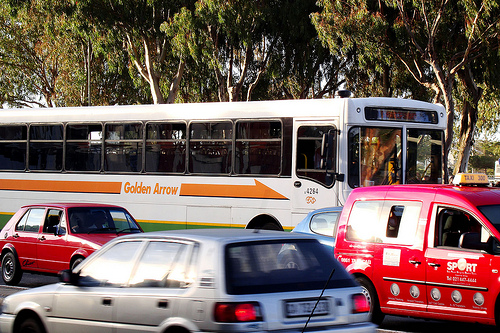
\includegraphics[width=.8\textwidth]{photos/trafficby_warrenski_flickr.jpg}\\
\textit{Foto deur warrenski op Flickr.}
\end{center}
\end{minipage}
   
\begin{enumerate}[noitemsep, label=\textbf{\arabic*}. ] 
    \item \textbf{posisie} of \textbf{verplasing} wat ons vertel van 'n voorwerp se ligging of verandering in ligging.
    \item \textbf{spoed} of \textbf{snelheid} wat vir ons vertel hoe vinnig 'n voorwerp beweeg en waarheen dit oppad is, en
    \item \textbf{versnelling} wat vir ons vertel hoe vinnig 'n voorwerp se spoed en snelheid verander. 
\end{enumerate}

\IFact{\textbf{Ruk} is die naam wat ons die verandering in versnelling noem.}


\section{Verwysingsraamwerk}
Die eerste ding op op te fokus wanneer jy die beweging van 'n voorwerp of persoon bestudeer is hulle posisie. Die woord \textsl{posisie} beskryf jou ligging (waar jy is). Dit help egter nie om te s\^e \textsl{hier} of \textsl{daar} nie, jy moet bekende liggings (verwysingspunte) gebruik om jou posisie te spesifiseer.

\begin{minipage}{.35\textwidth}
As jy byvoorbeeld in 'n klaskamer is en jy wil vir jou klasmaats vertel waar jy staan moet jy eers vir hulle 'n verwysingspunt gee. Die verwysingspunt kan dalk die klaskamer se deur wees. Jy sal dan kan se jy is 2~m van die deur af. Dit gee nie steeds nie jou presiese posisie nie. Jy sal 'n verwysingspunt en 'n koordinaatstelsel moet defini\"eer om jou presiese ligging te kan gee.
\end{minipage}
\begin{minipage}{.6\textwidth}
\begin{center}
\textbf{Beskrywing van jou posisie}\\
 \includegraphics[width=.8\textwidth]{photos/youarehereby_chokola_flickr.jpg}\\
\textit{Foto deur chokola op Flickr.}
\end{center}
\end{minipage}\\
Jy sal dan kan s\^e jy is, byvoorbeeld, 2~m weg van die deur aan die binnekant van die klaskamer. Die klaskamer se deur is 'n verywsingspunt en binne/buite is die koordinaatstelsel wat jy gekies het. 'n Verwysingsraamwerk is die verwysingspunt wat as die oorsprong van die koordinaatstelsel dien. Die koordinaatstelsel kan op of af, binne of buite, links of regs of selfs vorentoe en aftertoe wees. Hierdie is almal voorbeelde wat 'n 1 dimensionele koordinaatstelsel defini\"eer. Ons kies een van die rigtings as die \textbf{positiewe} rigting.

\Definition{Verwysingsraamwerk} {'n Verwysingsraamwerk is die verwysings punt gekombineer met 'n stel rigtings.} 
'n Grafiese tentoonstelling van 'n 1 dimensionele verwysingsraamwerk. 
\begin{figure}[H]
 \begin{center}
  \begin{pspicture}(-2,-2)(4,4)
   \psline{->}(-1,0)(3,0)
\rput(2,0.4){$\vec{x}_{i}$}
\rput(2,0){\qdisk(0,0){3pt}}
\rput(3.3,0){$x$}
\rput(0,-1.2){oorsprong}
\psdot(0,0)
\rput[l](.2,.8){positiewe (+) rigting}
\rput[r](-.2,.8){negatiewe (--) rigting}
\psline[linestyle=dashed](0,-1)(0,1)
  \end{pspicture}
 \end{center}
\caption{verwysingsraamwerk}
\label{fig:frameofref}
\end{figure}

Jy kan verskillende verwysingsraamwerke defini\"eer vir dieselfde probleem, maar die uitslag, die fisiese resultate, sal dieselfde wees. Byvoordeeld, 'n seun staan stil in 'n trein wanneer dit uit die stasie beweeg. Jy en die seun defini\"eer julle verwysingsraamwerk as julle eie huidige posisies en die rigting waarin die trein beweeg as die vorentoe rigting. 

Jy staan op die platform en kyk hoe die trein van links na regs beweeg. Vir jou lyk dit of die seun van links na regs beweeg, want relatief tot waar jy staan (die platform), is hy besig om te beweeg. Volgens die seun, en sy verwysingsraamwerk, staan hy stil.\par 
        
'n Verwysingsraamwerk moet 'n oorsprong h\^e (waar jy staan op die platform) en ten minste 'n positiewe rigting. Die trein het van links na regs beweeg, wat na regs positief maak en na jou linkerkant toe, negatief. As iemand anders na dieselfde seun gekyk het, sou hulle verwysingsraamwerk anders gewees het. As hy, byvoorbeeld, aan die ander kant van die platform gestaan het, sou die seun van regs na links beweeg het. \par

\begin{center}
\scalebox{1.3} % Change this value to rescale the drawing.
{
\begin{pspicture}(2.5,-1.5)(12.675,2.2879686)
%\psgrid
\psline[](4.26,-2.2479687)(4.26,-2.2479687)
\psline[](4.24,-2.1679688)(4.24,-2.1679688)
\psframe[linewidth=0.04,dimen=outer](5.06,0.47203124)(3.22,0.13203125)
\psframe[linewidth=0.04,dimen=outer](7.02,0.47203124)(5.18,0.13203125)
\psframe[linewidth=0.04,dimen=outer](9.06,0.47203124)(7.22,0.13203125)
\psline[](9.22,1.4920312)(9.22,0.17203125)
\psline[](0.0,1.6920313)(0.0,1.6920313)
\psline[](9.22,1.4720312)(10.02,1.4720312)
\psline[](10.02,1.4720312)(10.02,0.77203125)
\psline[](10.02,0.77203125)(11.22,0.77203125)
\psline[](11.22,0.77203125)(11.22,0.17203125)
\psline[](11.22,0.17203125)(9.22,0.17203125)
\psline[](10.42,1.4720312)(11.02,1.4720312)
\psline[](11.02,1.4720312)(10.82,0.77203125)
\psline[](10.42,1.4720312)(10.62,0.77203125)
\pscircle[linewidth=0.04,dimen=outer](9.82,-0.12796874){0.3}
\pscircle[linewidth=0.04,dimen=outer](10.72,-0.12796874){0.3}
\pscircle[linewidth=0.04,dimen=outer](8.52,-0.12796874){0.3}
\pscircle[linewidth=0.04,dimen=outer](7.62,-0.12796874){0.3}
\pscircle[linewidth=0.04,dimen=outer](6.52,-0.12796874){0.3}
\pscircle[linewidth=0.04,dimen=outer](5.62,-0.12796874){0.3}
\pscircle[linewidth=0.04,dimen=outer](4.62,-0.12796874){0.3}
\pscircle[linewidth=0.04,dimen=outer](3.72,-0.12796874){0.3}
\psline[linewidth=0.051999997cm](5.02,0.27203125)(5.22,0.27203125)
\psline[linewidth=0.05cm](7.02,0.27203125)(7.22,0.27203125)
\psline[linewidth=0.05cm](9.22,0.27203125)(9.02,0.27203125)
\rput{-14.036243}(-0.19131365,1.5252956){\psellipse[linewidth=0.05,dimen=outer](6.099412,1.5396783)(0.15764816,0.25)}
\psline[linewidth=0.05cm](6.04,1.3120313)(6.02,0.8720313)
\psline[linewidth=0.05cm](6.02,0.8720313)(5.82,0.47203124)
\psline[linewidth=0.05cm](5.82,0.47203124)(5.92,0.47203124)
\psline[linewidth=0.05cm](6.02,0.8720313)(6.02,0.45203125)
\psline[linewidth=0.05cm](6.02,0.47203124)(6.12,0.47203124)
\psline[linewidth=0.05cm](6.04,1.1720313)(5.92,0.97203124)
\psline[linewidth=0.05cm](5.92,0.97203124)(6.12,0.8720313)
\psdots[dotsize=0.12](6.18,1.5920312)
\psline[linewidth=0.05cm,]{->}(9.2,1.8920312)(10.62,1.8920312)

\rput(10.585781,2.1120312){\scriptsize trein beweeg van links na regs}

\rput(6.494219,2.1120312){\scriptsize seun staan stil}

\rput(7.5909376,-0.9479687){\scriptsize In jou verwysingsraamwerk beweeg die seun van links na regs.}
\psline[linewidth=0.05cm](6.02,1.1720313)(6.06,0.8720313)
\psline[linewidth=0.05cm](6.06,0.9320313)(6.1,0.7920312)
\pscustom[linewidth=0.05]
{
\newpath
\moveto(6.08,1.4920312)
\lineto(6.11,1.4620312)
\curveto(6.125,1.4470313)(6.145,1.4270313)(6.16,1.4120313)
}
\pscustom[linewidth=0.05]
{
\newpath
\moveto(6.24,1.8120313)
\lineto(6.12,1.7820313)
\curveto(6.06,1.7670312)(5.99,1.7520312)(5.96,1.7520312)
}
\pscustom[linewidth=0.05]
{
\newpath
\moveto(6.14,1.8120313)
\lineto(6.11,1.8120313)
\curveto(6.095,1.8120313)(6.075,1.8120313)(6.07,1.8120313)
\curveto(6.065,1.8120313)(6.05,1.7920313)(6.04,1.7720313)
\curveto(6.03,1.7520312)(6.015,1.7270312)(6.0,1.7120312)
}
\end{pspicture}  
}
\end{center}
\begin{center}
\begin{pspicture}(0,-0.5)(5,2)
%\psgrid[gridcolor=gray]
\pcline{<->}(0.5,0.5)(4.5,0.5)
\aput{:U}{\parbox[l]{4cm}{'n Seun binne in 'n trein wat van links na regs beweeg.}}
\psline(2.5,0.6)(2.5,0.4)
\uput[d](2.5,0.4){Waar jy staan}
\uput[d](2.5,0.0){op die platform}
\uput[d](2.5,-0.4){(verwysingspunt of oorsprong)}
\uput[r](4.5,0.5){positiewe rigting (na jou regterkant)}
\uput[l](0.5,0.5){negatiewe rigting (na jou linkerkant)}
\end{pspicture}
\end{center}

In hierdie hoofstuk sal ons net verwysingsraamwerke gebruik wat in die $x$ rigting is. Sodoende beperk ons onsself tot \textsl{een dimensionele beweging}. Ons kan die teken van die posisie-waarde (positief of negatief) gebruik om die rigting relatief tot die oorsprong te wys.

\Definition{Een dimensionele beweging}{'n Voorwerp se beweging word beperk tot 'n lyn.}

Byvoorbeeld, die blou kol in die figuur kan net op die $x$ as beweeg.
 \begin{center}
  \begin{pspicture}(-2,-2)(4,4)
   \psline[linewidth=.05cm]{<->}(-3,0)(3,0)
% \rput(2,0.4){$\vec{x}_{i}$}
\rput(2,0){\pscircle[linecolor=blue,fillcolor=blue,fillstyle=solid](0,0){.2}}
\rput(3.3,0){$x$}
\rput(0,-.2){oorsprong}
\psline(0,-.1)(0,.1)
  \end{pspicture}
 \end{center}
%Frames of reference will be covered in more detail in Grade 12.\par       
	
\begin{figure}[H] % horizontal\label{m38787*slidesharefigure}
    \label{m38787*slidesharemedia}\label{m38787*slideshareflash}\raisebox{-5 pt}{ 
\includegraphics[width=0.5cm]{col11305.imgs/summary_www.png}} { (Aanbieding:  P10097 )}
 \end{figure}       \par 
            

\subsection*{Posisie}
\nopagebreak

\Definition{Posisie} {Posisie is 'n mate van ligging, met verwysing na 'n oorsprong toe.\\
Simbool: $x$\hspace{2cm} S.I. Eenheid: m} 

'n Posisie is 'n mate van 'n ligging binne 'n verwysingsraamwerk. Dit beteken dat posisie negatief of positief kan wees afhangend van die keuse van die verwysingsraamwerk se koordinaatstelsel.

Afhangende van watter verwysingspunt ons kies, kan ons s\^e dat die skool $300~\text{m}$ van Kosma se huis is (met Kosma se huis as die verwysingspunt of oorsprong), of $500~\text{m}$ van Kevin se huis (met Kevin se huis as die verwysingspunt of oorsprong).\par
\begin{center}
\scalebox{1} % Change this value to rescale the drawing.
{
\begin{pspicture}(0,-1.421875)(14.005,1.386875)
\psframe[linewidth=0.05,dimen=outer](1.82,0.601875)(0.22,-0.298125)
\pstriangle[linewidth=0.05,dimen=outer](1.03,0.541875)(2.06,0.82)
\pstriangle[linewidth=0.05,dimen=outer](13.03,0.561875)(2.06,0.82)
\psline[linewidth=0.05cm,tbarsize=0.07055555cm 5.0]{|-|}(1.06,-0.918125)(13.1,-0.938125)
\psline[linewidth=0.05cm](3.08,-0.798125)(3.08,-1.038125)
\psline[linewidth=0.05cm](5.06,-0.798125)(5.06,-1.038125)
\psline[linewidth=0.05cm](7.06,-0.818125)(7.06,-1.038125)
\psline[linewidth=0.05cm](9.06,-0.798125)(9.06,-1.038125)
\psline[linewidth=0.05cm](11.06,-0.778125)(11.06,-1.018125)

\rput(2.085,-1.283125){\footnotesize $100 ~\text{m}$}
\psframe[linewidth=0.05,dimen=outer](13.86,0.621875)(12.26,-0.278125)
\psframe[linewidth=0.05,dimen=outer](3.62,0.581875)(2.54,-0.298125)
\psframe[linewidth=0.05,dimen=outer](5.6,0.581875)(4.52,-0.298125)
\psframe[linewidth=0.05,dimen=outer](7.6,0.581875)(6.52,-0.298125)
\psframe[linewidth=0.05,dimen=outer](9.62,0.581875)(8.54,-0.298125)
\psframe[linewidth=0.05,dimen=outer](11.62,0.581875)(10.54,-0.298125)
\pstriangle[linewidth=0.05,dimen=outer](3.08,0.521875)(1.36,0.54)
\pstriangle[linewidth=0.05,dimen=outer](7.06,0.521875)(1.36,0.54)
\pstriangle[linewidth=0.05,dimen=outer](5.04,0.521875)(1.36,0.54)
\pstriangle[linewidth=0.05,dimen=outer](9.06,0.521875)(1.36,0.54)
\pstriangle[linewidth=0.05,dimen=outer](11.08,0.521875)(1.36,0.54)

\rput(4.105,-1.263125){\footnotesize $100 ~\text{m}$}

\rput(6.105,-1.283125){\footnotesize $100 ~\text{m}$}

\rput(8.125,-1.263125){\footnotesize $100 ~\text{m}$}

\rput(10.125,-1.263125){\footnotesize $100 ~\text{m}$}

\rput(12.125,-1.283125){\footnotesize $100 ~\text{m}$}

\rput(13.068594,0.161875){\small Winkel}

\rput(1.065,0.171875){Skool}

\rput(3.0773437,0.171875){\small{Komal}}

\rput(5.0554686,0.171875){\small{Kholo}}

\rput(7.065469,0.171875){\small{Kosma}}

\rput(9.0725,0.171875){\small{Kogis}}

\rput(11.065469,0.171875){\small{Kevin}}
\end{pspicture} 
}
\end{center}

Die winkel is ook $300~m$ can Kosma se huis af, maar in die teenoorgestelde rigting as die skool. Wanneer ons 'n verwysingspunt kies, het ons 'n positiewe en negatiewe rigting. As ons die rigting na die skool toe as negatief kies, dan is die rigting na die winkel toe positief. 'n Negatiewe rigting is altyd in die teenoorgestelde rigting as die rigting wat as positief gekies is. 
    
\begin{center}
\scalebox{1} % Change this value to rescale the drawing.
{
\begin{pspicture}(0,-1.1871876)(9.225,1.1871876)
\psline[linewidth=0.05cm,]{<->}(0.0,-0.6428125)(8.0,-0.6428125)
\psline[linewidth=0.05cm](1.02,-0.5028125)(1.02,-0.7828125)
\psline[linewidth=0.05cm](2.02,-0.5028125)(2.02,-0.7828125)
\psline[linewidth=0.05cm](3.0,-0.5028125)(3.0,-0.7828125)
\psline[linewidth=0.05cm](4.02,-0.5028125)(4.02,-0.7828125)
\psline[linewidth=0.05cm](5.02,-0.5028125)(5.02,-0.7828125)
\psline[linewidth=0.05cm](6.02,-0.5028125)(6.02,-0.7828125)
\psline[linewidth=0.05cm](7.02,-0.5028125)(7.02,-0.7828125)

\rput(0.97625,-1.0328125){$-300$}

\rput(1.97625,-1.0328125){$-200$}

\rput(2.97625,-1.0328125){$-100$}

\rput(3.9970312,-1.0128125){$0$}

\rput(5.0025,-1.0128125){$+100$}

\rput(6.0196877,-1.0128125){$+200$}

\rput(7.01625,-1.0128125){$+300$}
\psline[linewidth=0.05cm,]{->}(1.0,0.2971875)(1.0,-0.4428125)
\psline[linewidth=0.05cm,]{->}(4.02,0.3171875)(4.02,-0.4628125)
\psline[linewidth=0.05cm,]{->}(7.02,0.2971875)(7.02,-0.4828125)

\rput(0.965,0.6871875){Skool}

\rput(4.101094,1.0071875){Kosma se huis}

\rput(4.1451564,0.6071875){(verwysingspunt)}

\rput(7.012656,0.6871875){Winkel}

\rput(8.612968,-0.5928125){$x$ (m)}
\end{pspicture}  }
\end{center}

Die oorsprong is by Kosma se huis en die posisie van die skool is $-300~\text{m}$. Posisies na links word gedefini\"eer as negatief en posisies na regs as positief.

Neem kennis dat ons ook die rigting na die skool as positief kan kies. In hierdie geval is Kosma se huis nog steeds $300~m$ van die skool af, maar dit is nou in die positiewe rigting.

\begin{center}
\scalebox{1} % Change this value to rescale the drawing.
{
\begin{pspicture}(0,-1.1871876)(9.225,1.1871876)
\psline[linewidth=0.05cm,]{<->}(0.0,-0.6428125)(8.0,-0.6428125)
\psline[linewidth=0.05cm](1.02,-0.5028125)(1.02,-0.7828125)
\psline[linewidth=0.05cm](2.02,-0.5028125)(2.02,-0.7828125)
\psline[linewidth=0.05cm](3.0,-0.5028125)(3.0,-0.7828125)
\psline[linewidth=0.05cm](4.02,-0.5028125)(4.02,-0.7828125)
\psline[linewidth=0.05cm](5.02,-0.5028125)(5.02,-0.7828125)
\psline[linewidth=0.05cm](6.02,-0.5028125)(6.02,-0.7828125)
\psline[linewidth=0.05cm](7.02,-0.5028125)(7.02,-0.7828125)

\rput(0.97625,-1.0328125){$+300$}

\rput(1.97625,-1.0328125){$+200$}

\rput(2.97625,-1.0328125){$+100$}

\rput(3.9970312,-1.0128125){$0$}

\rput(5.0025,-1.0128125){$-100$}

\rput(6.0196877,-1.0128125){$-200$}

\rput(7.01625,-1.0128125){$-300$}
\psline[linewidth=0.05cm,]{->}(1.0,0.2971875)(1.0,-0.4428125)
\psline[linewidth=0.05cm,]{->}(4.02,0.3171875)(4.02,-0.4628125)
\psline[linewidth=0.05cm,]{->}(7.02,0.2971875)(7.02,-0.4828125)

\rput(0.965,0.6871875){Skool}

\rput(4.101094,1.0071875){Kosma se huis}

\rput(4.1451564,0.6071875){(verwysingspunt)}

\rput(7.012656,0.6871875){Winkel}

\rput(8.612968,-0.5928125){$x$ (m)}
\end{pspicture}  }

\end{center}

Die oorsprong is by Kosma se huis en die posisie van die skool is $+300~\text{m}$. Posisies na links word as positief gedefini\"eer en posisies na regs as negatief.

\begin{groupdiscussion}{Verwysingspunte}
            \nopagebreak
Deel op in groepe van 5 vir hierdie aktiwiteit. Kies 'n verwysingspunt vir 'n reguit lyn. Omdat posisie beide negatiewe en positiewe waardes kan h\^e, bespreek die voor- en nadele as jy die verwysingspunt kies as:
\begin{enumerate}[noitemsep, label=\textbf{\arabic*}. ] 
    \item een kant van die lyn
    \item die middel van die lyn. (Hierdie verwysingspunt kan ook die ``oorsprong'' genoem word.)
\end{enumerate}
Staan in 'n reguit lyn, maak beurte om verskillende mense in jou groep te kies as die oorsprong. Laat die persoon wat die oorsprong is toe om die positiewe rigting te kies. Elkeen behoort dan te probeer om hulle posisies te defini\"eer. Die posisies hoef nie baie presies te wees nie maar jy kan 'n benadering maak. Dit is belangrik om te verstaan hoekom jou posisie positief of negatief is vir elke verskillende oorsprong en koordinaatstelsel.

Neem kennis dat jou posisie elke keer verskillend is maar dat jy nie beweeg het nie. Die manier hoe 'n antwoord geskryf word kan deur die koordinaatstelsel be\"invloed word maar fisiese prosesse behoort nooit be\"invloed te word nie.
\end{groupdiscussion}

\begin{exercises}{Posisie}
\begin{enumerate}[noitemsep, label=\textbf{\arabic*}. ] 
    \item Skryf die posisies neer van voorwerpe by A, B, D en E. Moenie die eenhede vergeet nie.
\begin{figure}[H] % horizontal\label{m38787*id62877}
\begin{center}
\begin{pspicture*}(-6,-1)(6.1,1)
\psset{dotsize=7pt}
%\psgrid[gridcolor=lightgray]
\multirput(0,0)(0,0){1}{
\multido{\n=-4+1}{9}
{\psline{<->}(-5,0)(5,0)
\rput(\n,0){\psline(0,-0.1)(0,0.1)}
\uput[d](\n,-0.1){\n}}
\uput[r](5,0){$x$ (m)}}
\uput[u](0,0.5){verwysingspunt}
\uput[u](-3,0.2){A}
\uput[u](-1,0.2){B}
\uput[u](1,0.2){D}
\uput[u](3,0.2){E}
\psline{->}(0,0.6)(0,0.2)
\end{pspicture*}
\end{center}
 \end{figure}

\item Skryf die posisies neer van voorwerpe by F,G,H en J. Moenie die eenhede vergeet nie.
\begin{figure}[H] % horizontal\label{m38787*id62899}
\begin{center}
\begin{pspicture*}(-6,-1)(6.1,1)
\psset{dotsize=7pt}
%\psgrid[gridcolor=lightgray]
\multirput(0,0)(0,0){1}{
\multido{\n=-4+1}{9}
{\psline{<->}(-5,0)(5,0)
\rput(\n,0){\psline(0,-0.1)(0,0.1)}
\uput[d](-\n,-0.1){\n}}
\uput[r](5,0){$x$ (m)}}
\uput[u](0,0.5){verwysingspunt}
\uput[u](-3,0.2){F}
\uput[u](-1,0.2){G}
\uput[u](1,0.2){H}
\uput[u](3,0.2){J}
\psline{->}(0,0.6)(0,0.2)
\end{pspicture*}
\end{center}
 \end{figure}

\item Daar is 5 huise op Newton straat, A, B, C, D en E. Neem aan die posisies na regs is positief.
\begin{figure}[H] % horizontal\label{m38787*id62920}
\begin{center}
\begin{pspicture*}(-4.2,-0.2)(5.2,2.8)
\def\house{\psframe(0,0)(1,1)\pspolygon(0,1)(0.5,2)(1,1)}
\def\distance{\psline(0.5,2.2)(0.5,2.4)\psline(2.5,2.2)(2.5,2.4)\psline{<->}(0.5,2.3)(2.5,2.3)\uput[u](1.5,2.3){20 m}}
\psset{dotsize=7pt}
%\psgrid[gridcolor=lightgray]
\multirput(-4,0)(2,0){5}{\house}
\multirput(-4,0)(2,0){4}{\distance}
\rput(-3.5,0.5){\Large{\textsf{A}}}
\rput(-1.5,0.5){\Large{\textsf{B}}}
\rput(0.5,0.5){\Large{\textsf{C}}}
\rput(2.5,0.5){\Large{\textsf{D}}}
\rput(4.5,0.5){\Large{\textsf{E}}}
\end{pspicture*}
\end{center}
 \end{figure}       
 
\begin{enumerate}[noitemsep, label=\textbf{\alph*}. ] 
    \item Teken 'n verwysingsraamwerk met huis A as oorsprong en skryf dan die posisies neer van huise B, C, D en E.
    \item Jy bly in huis C. Wat is jou posisie relatief tot huis E?
    \item Wat is die posisies van huise A, B en D as huis B as die verwysingspunt gekies word?
\end{enumerate}
\end{enumerate}

\par \raisebox{-5 pt}{
\includegraphics[width=0.5cm]{col11305.imgs/summary_www.png}} Vind antwoorde met die kortkodes: 
 \par \begin{tabular}[h]{cccccc}
 (1.) laG  &  (2.) la7  &  (3.) laA  & \end{tabular}
\end{exercises}

\subsection*{Verplasing en afstand}
    \nopagebreak
%            \label{m38788} $ \hspace{-5pt}\begin{array}{cccccccccccc}   \end{array} $ \hspace{2 pt}\raisebox{-5 pt}{
\includegraphics[width=0.5cm]{col11305.imgs/summary_www.png}} {(section shortcode: P10098 )} \par 
\Definition{Verplasing}{ Verplasing is die verandering in 'n voorwerp se posisie. Dit is 'n vektor van die oorspronklike posisie ($\vec{x}_{i}$) na die finale posisie ($\vec{x}_{f}$) wys.\par
Simbool: $\Delta \vec{x}$\hspace{2cm} S.I. Eenheid: $\text{m}$ }

Die verplasing van 'n voorwerp word gedefini\"eer as die verandering in posisie (finale posisie minus aanvanklike posisie). Verplasing het 'n grootte en 'n rigting en is dus 'n vektor. Byvoorbeeld, as die aanvanklike posisie van 'n kar $\vec{x}_{i}$ is en dit beweeg na 'n finale posisie $\vec{x}_{f}$, dan is die verplasing:

\Tip{Die simbool $\Delta $ word gelees as \textsl{delta}. $\Delta $ is 'n letter van die Griekse alfabet en word in Wiskunde en Wetenskap gebruik om 'n verandering van 'n hoeveelheid, of finale waarde minus aanvanklike waarde, aan te dui. Byvoorbeeld, $\Delta x$ beteken verandering in $x$ terwyl $\Delta t$ verandering in $t$ aandui.}
        
\begin{equation*}
    \vec{x}_{f}-\vec{x}_{i}
  \end{equation*}
Dit help om die verplasing te visualiseer as jy terug dink aan die stert-na-kop metode. Die verplasing is die vektor wat jy by die aanvanklike posisie tel om die finale posisie te kry.

In Fisika gebruik ons egter die kortpad $\Delta$ om aan te dui dat ons 'n aanvanklike posisie van 'n finale een afgetrek het,     dus skryf ons: 
\begin{equation*}
    \Delta \vec{x}=\vec{x}_{f}-\vec{x}_{i}
\end{equation*}


Die volgende diagram illustreer die konsep van verplasing:
\begin{figure}[H]
 \begin{center}
  \begin{pspicture}(-2,-2)(5,5)
   \psline{<->}(-1,0)(4,0)
\rput(1,0){\qdisk(0,0){2pt}}
\rput(3,0){\qdisk(0,0){2pt}}
\rput[t](0,0.5){$0$}
\psline(0,-.2)(0,.2)
\rput[t](1,0.5){$\vec{x}_{i}$}
\rput[t](3,0.5){$\vec{x}_{f}$}
\psline{->}(1,-.3)(3,-0.3)
\rput[b](2,-.7){$\Delta \vec{x}$}
  \end{pspicture}
 \end{center}
\end{figure}
As jy byvoorbeeld 'n bal $5~\text{m}$ ver in 'n reguit lyn rol is sy verplasing $5~\text{m}$, indien jy die rigting waarin die bal rol as positief vat en die aanvanklike posisie as $0~\text{m}$.

\Tip{Die woorde \textsl{aanvanklik} end \textsl{finaal} word dikwels in Fisika gebruik. \textsl{Aanvanklik} verwys na die situasie aan die begin van die beskrywing/probleem en \textsl{finaal} na die situasie aan die einde. Dit gebeur ook dikwels dat die finale waarde kleiner as die aanvanklike waarde is wat maak dat die verskil negatief is. Dit is nie 'n probleem nie!}
     
Verplasing is nie afhanklik van die pad wat gevolg word nie, net die aanvaklike en finale posisies. Ons gebruik die woord \textsl{afstand} as ons wil beskryf hoe ver 'n voorwerp op 'n sekere pad beweeg het.

\Tip{Ons sal $D$ in hierdie boek gebruik, maar jy sal dalk $d$ in ander boeke sien.}

\Definition{Afstand}{Afstand is die totale lengte van die pad wat gevolg word van die aanvanklike posisie, $\vec{x}_{i}$, na die finale posisie, $\vec{x}_{f}$. Afstand is 'n skalaar.\\Simbool: $D$\hspace{2cm} S.I. Eenheid: $\text{m}$}

In die diagram hieronder kan jy sien dat die pad kronkel as gevolg van heuwels vanaf 'n skool na 'n nabye winkel. Die pad word as 'n strepieslyn aangedui. \\

\begin{minipage}{.5\textwidth}
Afstand is die lengte van die strepieslyn. Dit is hoe very jy sal moet stap as jy die pad volg. Die verplasing is anders. Verplasing is die reguit lyn van die beginpunt tot by die eindpuny -- van die skool na die winkel soos aangedui met die pyl in die figuur.
\end{minipage}
\begin{minipage}{.5\textwidth}
\begin{center}
\begin{pspicture}(0.2,0.2)(5,5)
%\psgrid[gridcolor=lightgray]
\psdots(0.5,1)\psdots(4.5,1)
\pscurve[linestyle=dashed,linecolor=blue](0.5,1)(1,1.5)(2,2.5)(2.5,0)(4,2)(4.5,1)
\rput(0.5,0.7){Begin}
\rput(0.5,0.3){(Skool)}
\rput(4.5,0.7){Einde}
\rput(4.5,0.3){(Winkel)}
% \psline[linewidth=0.05, linestyle=dotted, arrowscale=2]{->}(0.5,1)(4.4,1)
% \psline[linewidth=0.05, linestyle=dotted,arrowscale=2]{->}(4.4,1)(4.4,4.4)
\pcline[arrowscale=2]{->}(0.5,1)(4.5,1)
% \lput*{:U}{Displacement}
\end{pspicture}
\end{center}
\end{minipage}
\Tip{Ons gebruik die uitdrukking \textsl{'soos die kraai vlieg'} om 'n reguit lyn tussen twee punte te beskryf, omdat vo\"els reguit oor hindernisse kan vlieg.}

\subsubsection*{Illustrasie van verplasing en afstand}
As ons dieselfde situasie as vantevore gebruik kan ons die konsep in meer detail bestudeer. Beskou ons beskrywing van die ligging van die huise, die skool en die winkel.

\begin{figure}
\centering
\scalebox{1} % Change this value to rescale the drawing.
{
\begin{pspicture}(0,-1.421875)(14.005,1.386875)
\psframe[linewidth=0.05,dimen=outer](1.82,0.601875)(0.22,-0.298125)
\pstriangle[linewidth=0.05,dimen=outer](1.03,0.541875)(2.06,0.82)
\pstriangle[linewidth=0.05,dimen=outer](13.03,0.561875)(2.06,0.82)
\psline[linewidth=0.05cm,tbarsize=0.07055555cm 5.0]{|-|}(1.06,-0.918125)(13.1,-0.938125)
\psline[linewidth=0.05cm](3.08,-0.798125)(3.08,-1.038125)
\psline[linewidth=0.05cm](5.06,-0.798125)(5.06,-1.038125)
\psline[linewidth=0.05cm](7.06,-0.818125)(7.06,-1.038125)
\psline[linewidth=0.05cm](9.06,-0.798125)(9.06,-1.038125)
\psline[linewidth=0.05cm](11.06,-0.778125)(11.06,-1.018125)

\rput(2.085,-1.283125){\footnotesize $100 ~\text{m}$}
\psframe[linewidth=0.05,dimen=outer](13.86,0.621875)(12.26,-0.278125)
\psframe[linewidth=0.05,dimen=outer](3.62,0.581875)(2.54,-0.298125)
\psframe[linewidth=0.05,dimen=outer](5.6,0.581875)(4.52,-0.298125)
\psframe[linewidth=0.05,dimen=outer](7.6,0.581875)(6.52,-0.298125)
\psframe[linewidth=0.05,dimen=outer](9.62,0.581875)(8.54,-0.298125)
\psframe[linewidth=0.05,dimen=outer](11.62,0.581875)(10.54,-0.298125)
\pstriangle[linewidth=0.05,dimen=outer](3.08,0.521875)(1.36,0.54)
\pstriangle[linewidth=0.05,dimen=outer](7.06,0.521875)(1.36,0.54)
\pstriangle[linewidth=0.05,dimen=outer](5.04,0.521875)(1.36,0.54)
\pstriangle[linewidth=0.05,dimen=outer](9.06,0.521875)(1.36,0.54)
\pstriangle[linewidth=0.05,dimen=outer](11.08,0.521875)(1.36,0.54)

\rput(4.105,-1.263125){\footnotesize $100 ~\text{m}$}

\rput(6.105,-1.283125){\footnotesize $100 ~\text{m}$}

\rput(8.125,-1.263125){\footnotesize $100 ~\text{m}$}

\rput(10.125,-1.263125){\footnotesize $100 ~\text{m}$}

\rput(12.125,-1.283125){\footnotesize $100 ~\text{m}$}

\rput(13.068594,0.161875){\small Winkel}

\rput(1.065,0.171875){Skool}

\rput(3.0773437,0.171875){\small{Komal}}

\rput(5.0554686,0.171875){\small{Kholo}}

\rput(7.065469,0.171875){\small{Kosma}}

\rput(9.0725,0.171875){\small{Kogis}}

\rput(11.065469,0.171875){\small{Kevin}}
\end{pspicture} 
}
\caption{}
\label{position:reference3}
\end{figure}
Komal stap om vir Kevin by sy huis te ontmoet voor hulle skool toe stap. Wat is Komal se verplasing en wat is die afstand wat hy moet stap as hy skool toe stap via Kevin se huis?

Komal l\^e 'n afstand van $400~m$ af na Kevin se huis toe en nog $500~m$ van Kevin se huis na die skool. Hy l\^e dus 'n totale afstand van $900~m$ af. Sy verplasing is egter net $100~m$ na die skool toe. Die rede is omdat verplasing net die beginpunt (sy huis) en die eindpunt (die skool) in ag neem. Dit is nie afhanklik van die roete wat hy geneem het nie.

Om die afstand en verplasing te bereken moet ons 'n verwysingspunt en 'n rigting kies. Kom ons kies Komal se huis as die verwysingspunt en die rigting na Kevin se huis as die positiewe rigting (dit beteken die rigting na die skool toe is negatief). Ons doen die berekeninge dan as volg:\par 
\begin{minipage}{0.35\textwidth}
\begin{eqnarray*}
\text{Afstand (D)} &=& \text{roete gevolg}\\
&=&400\ \text{m} + 500\ \text{m}\\
&=&900\ \text{m}\\
\end{eqnarray*}
\end{minipage}
\begin{minipage}{0.65\textwidth}
\begin{eqnarray*}
\text{Verplasing} (\Delta \vec{x}) &=& \vec{x}_f~ - ~ \vec{x}_i\\
&=&-100\ \text{m} + 0\ \text{m}\\
&=&-100\ \text{m}\\
&=&100\ \text{m} \text{( in ~die~ negatiewe~} x \text{~rigting)}
\end{eqnarray*}
\end{minipage}\par


Jy sal gereeld negatiewe antwoorde in jou berekeninge kry. Byvoorbeeld, Komal se verplasing in die voorbeeld hierbo is as $-100~m$ bereken. Die minus teken voor die antwoord wys dat sy verplasing $100~m$ in die teenoorgestelde rigting (teenoorgestelde rigting as die rigting wat as positief gekies is) is. Wanneer ons 'n berekening begin, kies ons 'n verwysingsraamwerk en 'n positiewe rigting. In die eerste voorbeeld hierbo was dit verwysingspunt Komal se huis en die positiewe rigting was na Kevin se huis toe. Komal se verplasing is dus $100~m$ na die skool toe. Neem kennis dat afstand nie 'n rigting het nie maar verplasing het wel.\par


Kevin stap skool toe saam met Komal en na skool loop hy terug huis toe. Wat is Kevin se verplasing en watter afstand het hy afgel\^e? Vir hierdie berekening gebruik ons Kevin se huis as die verwysingspunt. Kom ons neem aan die rigting na die skool toe is positief.\\
\begin{minipage}{0.5\textwidth}
\begin{eqnarray*}
\text{Afstand (D)} &=& \text{roete~gevolg}\\
&=&500\ \text{m} + 500\ \text{m}\\
&=&1000\ \text{m}
\end{eqnarray*}
\end{minipage}
\begin{minipage}{0.5\textwidth}
\begin{eqnarray*}
\text{Verplasing} (\Delta \vec{x}) &=& \vec{x}_f~ - ~ \vec{x}_i\\
&=&0\ \text{m} + 0\ \text{m}\\
&=&0\ \text{m}
\end{eqnarray*}
\end{minipage} 
\par
Dit is moontlik om 'n verplasing van $0~m$ te h\^e en 'n afstand wat nie $0~m$ is nie. Dit gebeur wanneer jy eindig waar jy begin het.

\subsubsection*{Die verskil tussen afstand en verplasing}
            \nopagebreak
Die verskille tussen afstand en verplasing kan as volg opgesom word:\par
\begin{center}
\begin{tabular}{|l|l|}\hline
\textbf{ Afstand} & \textbf{ Verplasing} \\\hline
1. Afhanklik van roete & 1. Onafhanklik van roete \\\hline
2. altyd positief & 2. negatief of positief \\\hline
3. is 'n skalaar & 3. is 'n vektor\\\hline
\end{tabular}
\end{center}
    \par
\label{m38788*secfhsst!!!underscore!!!id498}
\begin{exercises}{Verwysingsraamwerke, verplasing en afstand}
\nopagebreak \noindent
\begin{enumerate}[noitemsep, label=\textbf{\arabic*}. ] 
\item Gebruik Figuur~\ref{position:reference3} om die volgende te beantwoord.
\begin{enumerate}[noitemsep, label=\textbf{\alph*}. ] 
    \item Kogis stap na Kosma se huis en dan skool toe. Wat is haar afstand en verplasing?
    \item Kholo stap na Kosma se huis en dan skool toe. Wat is haar afstand en verplasing?
    \item Komal stap winkel en daarna skool toe.i Wat is sy afstand en verplasing?
    \item Watter verwysingspunt het jy vir elk van die vrae gebruik?
\end{enumerate}
                
\item Jy staan by die voordeur van jou huis (verplasing, $\Delta \vec{x}=0~\text{m}$). Die straat is $10~\text{m}$ van die voordeur af. Jy stap na die straat toe en terug.
\begin{enumerate}[noitemsep, label=\textbf{\alph*}. ] 
    \item Wat is die afstand wat jy gestap het?
    \item Wat is jou finale verplasing?
    \item Is verplasing 'n vektor of 'n skalaar? Gee redes vir jou antwoord.
\end{enumerate}
\end{enumerate}
  \label{m38788**end}
\par \raisebox{-5 pt}{
\includegraphics[width=0.5cm]{col11305.imgs/summary_www.png}} Vind antwoorde met die kortkodes:
 \par \begin{tabular}[h]{cccccc}
 (1.) lDl  &  (2.) las  & \end{tabular}
\end{exercises}



\section{Spoed and snelheid} 
    \nopagebreak

\Definition{Gemiddelde spoed}
{Gemiddelde spoed is die \textbf{afstand} ($D$) afgel\^e gedeel deur die tyd ($\Delta t$) wat die reis geneem het.\\
Simbool: $v_{av}$\hspace{2cm} S.I. Eenhede: $\text{m}\cdot \text{s}^{-1}$} 


\Definition{Gemiddelde snelheid}{Gemiddelde snelheid is die \textbf{verplasing} van 'n liggam gedeel deur die tyd wat dit geneem het vir die verplasing om te gebeur.\\
Simbool: $\vec{v}_{av}$\hspace{2cm} S.I. Eenhede: $\text{m}\cdot \text{s}^{-1}$} 

Neem kennis dat die gemiddelde spoed 'n groot waarde kan h\^e terwyl die gemiddelde snelheid nul is.

Gemiddelde snelheid is die tempo waarteen posisie verander. Dit s\^e vir ons hoeveel 'n voorwerp se se posisie verander in 'n eenheid van tyd. Snelheid is 'n vektor. Ons gebruik die simbool $\vec{v}_{av}$ vir gemiddelde snelheid. As ons 'n verplasing het van $\Delta \vec{x}$ en 'n tyd geneem van $\Delta t$ word $\vec{v}_{av}$ dan gedefini\"eer as:\par 
\begin{eqnarray*}
\text{gemiddelde snelheid (in m} \cdot \text{s}^{-1}) &=& \frac{\text{verandering in verplasing (in m)}}{\text{verandering in tyd (in s)}}\\
\vec{v}_{av} &=& \frac{\Delta \vec{x}}{\Delta t}
\end{eqnarray*}\label{eq:pr:velocity}
Snelheid kan positief of negatief wees. 'n Positiewe snelheid wys in die rigting wat jy as positief gekies het in jou koordinaatstelsel. 'n Negatiewe snelheid wys in die teenoorgestelde rigting as die positiewe rigting.

Gemiddelde spoed (simbool $v_{av}$) is die afstand wat afgel\^e is ($D$), gedeel deur die tyd ($\Delta t$) wat dit geneem het om die afstand af te \^e. Afstand en tyd is skalare en dus is spoed ook 'n skalaar. Spoed word as volg bereken:\par 
        
\begin{equation*}
\text{gemiddelde spoed (in m} \cdot {\text{s}}^{-1}\text{)}  =  \frac{\text{afstand (in m)}}{\text{tyd (in s)}} 
\end{equation*}
\label{m38791*id64639}\nopagebreak\noindent{}
\begin{equation*}
v_{av}=\frac{D}{\Delta t}
\end{equation*}
     

 
\begin{wex}{Gemiddelde spoed en snelheid}
{James stap $2 \text{ km}$ van sy huis af in 30 minute. Hy draai dan om en stap huis toe volgens dieselfde roete, ook in 30 minute. Bereken James se gemiddelde spoed en gemiddelde snelheid.\\
\begin{center}
\begin{pspicture}(0,0)(3,0.5)
%\psgrid
\psline[linewidth=1pt]{->}(0,0)(2,0)
\psline[linewidth=1pt]{->}(2,0.5)(0,0.5)
% \psarc[linewidth=1pt]{->}(2.1,0.25){0.25}{-90}{90}
\uput[d](1,1){$2 \text{ km}$}
\end{pspicture}
\end{center}}
{

\westep{Identifiseer watter inligting gegee is en wat verlang word.}
Die vraag gee uitdruklik
\begin{itemize}
    \item die afstand en tyd daarheen ($2\text{ km}$ in 30 minute)
    \item die afstand en tyd terug ($2\text{ km}$ in 30 minute)
\end{itemize}

\westep{Maak seker dat alle eenhede SI eenhede is}
Die informasie is nie in SI eenhede nie en moet dus omgeskakel word.\\
Om km na m om te skakel weet ons dat:
\begin{eqnarray*}
1\ \text{km} &=&1\ 000\ \text{m}\\
\therefore\quad 2\ \text{km} &=&2\ 000\ \text{m} \quad \text{(vermenigvuldig albei kante met $2$.)}
\end{eqnarray*}
Op 'n soortgelyke manier kan ons 30 minute na sekondes omskakel
\begin{eqnarray*}
1\ \text{min} &=&60 \text{s}\\
\therefore\quad 30\ \text{min} &=&1\ 800\ \text{s} \quad \mbox{(vermenigvuldig albei kante met 30)}
\end{eqnarray*}

\westep{Bereken James se verplasing en afstand}
James het by die huis begin en teruggekeer huis toe, sy verplasing is dus 0 m.
$\Delta \vec{x} = 0\ \text{m}$\\
James het 'n totale afstand van $4 000 \text{ m}$ ($2\ 000\text{ m}$ daarheen en $2\ 000\text{ m}$ terug).\\
$D = 4\ 000\;\text{m}$
 
\westep{Bereken sy totale tyd}
James het $1~800\text{ s}$ geneem om daarheen te stap en $1~800\text{ s}$ om terug te stap.\\
$\Delta t = 3\ 600\;\text{s}$

\westep{Bereken sy gemiddelde spoed}
\begin{eqnarray*}
v_{av}&=&\frac{D}{\Delta t}\\
&=&\frac{4\ 000\ \text{m}}{3\ 600\ \text{s}}\\
&=&1,11\ ~\text{m}\cdot \text{s}^{-1}
\end{eqnarray*}

\westep{Bereken sy gemiddelde snelheid}
\begin{eqnarray*}
{\vec{v}_{av}}&=&\frac{\Delta \vec{x}}{\Delta t}\\
&=&\frac{0\ \text{m}}{3\ 600\ \text{s}}\\
&=& 0\ ~\text{m}\cdot \text{s}^{-1}
\end{eqnarray*}}
\end{wex}


\subsection*{Die verskil tussen sped en snelheid}
Die verskille tussen spoed en snelheid kan as volg opgesom word:\par
\begin{center}
\begin{tabular}{|p{5cm}|p{5cm}|}\hline
\textbf{Spoed} & \textbf{Snelheid} \\\hline
1. afhanklik van die roete & 1. onafhanklik van die roete \\\hline
2. altyd positief & 2. kan positief of negatief wees \\\hline
3. is 'n skalaar & 3. is 'n vektor \\\hline
4. onafhanklik van rigting en is dus positief & 4. rigting kan bepaal word van die teken (d.w.s. positief of negatief) \\\hline
\end{tabular}
\end{center}
    \par
Daarbenewens kan 'n voorwerp 'n op 'n plek begin en terugkeer na dieselfde plek en 'n snelheid van 0 h\^e maar 'n teen 'n nie-nul spoed beweeg. \par

\begin{exercises}{Verplasing en verwante hoeveelhede} \noindent
\nopagebreak
\begin{enumerate}[noitemsep, label=\textbf{\arabic*}. ] 
    \item Bongani moet winkel toe stap om melk te koop. Nadat hy $100~\text{m}$ gestap het kom hy agter hy het nie genoeg geld gebring nie en stap terug huis toe. As dit hom twee minute geneem het om die huis te verlaat en terug te keer, bereken die volgende:
    \begin{enumerate}[noitemsep, label=\textbf{\alph*}. ] 
        \item Hoe lank wys hy buite die huis (die tydsinterval $\Delta t$ in sekondes)?
        \item Hoe ver het hy gestap (afstand ($D$))?
        \item Wat was sy verplasing ($\Delta \vec{x}$)?
        \item Wat was sy gemiddelde snelheid (in $\text{m} \cdot \text{s}^{-1}$)?
        \item Wat was sy gemiddelde spoed (in $\text{m} \cdot \text{s}^{-1}$)?
\end{enumerate}
	
\begin{figure}[H] % horizontal\label{m38791*id66785}
\begin{center}
\scalebox{0.5} % Change this value to rescale the drawing.
{
\begin{pspicture}(0,-3.7525)(6.5721874,3.7325)
\psline[]{->}(5.4625,-2.4475)(-5.8225,-2.4675)
\psline[]{->}(-5.8825,-2.7875)(5.4625,-2.7875)
\rput(0,-3.1575){\huge 100 m}
\rput(0,-1.3){\huge 2 minute daarheen en terug}
\rput(0,-2){\huge $100 \text{ m}$}
\rput(6.53625,-2.5975){\huge huis}
\rput(-6.70765626,-2.5975){\huge winkel}
\end{pspicture} 
}
\end{center}
\end{figure}

\item Bridget kyk na 'n reguit stuk pad vanuit haar klaskamer se venster. Sy kan twee pale sien wat sy vroe\"er gemeet het as $50\text{ m}$ van mekaar af. Sy gebruik haar stophorlosie om te meet dat meeste karre $3 \text{ s}$ neem om van een paal na die volgende te ry.
\begin{enumerate}[noitemsep, label=\textbf{\alph*}. ] 
    \item Gebruik die vergelyking vir snelheid, ($\vec{v}_{av}$ = $\frac{\Delta \vec{x}}{\Delta t}$), en wys al die stappe wat nodig is om die snelheid van 'n kar te bereken wat van links na regs beweeg.
    \item As Bridget die snelheid van 'n rooi Golf meet as $-16,67~\text{m}\ensuremath{\cdot}\text{s}{}^{-1}$, in watter rigting beweeg die Golf?\par
    Bridget los haar stophorlosie aan en sien dat 'n taxi by $t=5,0~\text{s}$ verby die linkerkantste paal ry en 'n bus wat terselfdertyd verby die regterkantste paal ry. By die tyd $t=7,5~\text{s}$ ry die taxi verby die regterkantste paal. Wanneer die tyd $t=9,0~\text{s}$ is, ry die bus verby die linkerkantste paal.
    \item Hoe lank het dit die taxi en die bus geneem om tussen die twee pale te ry? (Bereken die tydsinterval ($\Delta t$) vir beide die taxi en die bus).
    \item Wat was die gemiddelde snelheid van die taxi en die bus?
    \item Wat was die gemiddelde spoed van die taxi en die bus?
    \item Wat was die gemiddelde spoed van die taxi en die bus in $\text{km}\ensuremath{\cdot}\text{h}{}^{-1}$?
\end{enumerate}
	\begin{figure}[H] % horizontal\label{m38791*id66998}
\begin{center}
\scalebox{1} % Change this value to rescale the drawing.
{
\begin{pspicture}(0,-3.22)(6.74,3.2)
\psframe[linewidth=0.04,dimen=outer](1.12,3.2)(1.02,0.2)
\psframe[linewidth=0.04,dimen=outer](5.22,3.2)(5.12,0.2)
\psline[]{<->}(1.12,0.3)(5.12,0.3)

\rput(3.080625,0.61){50 m}
\psline[](0.82,-0.4)(1.12,-0.5)
\psline[](1.12,-0.5)(1.12,-0.7)
\psline[](1.12,-0.7)(0.92,-0.7)
\psline[](0.72,-0.7)(0.42,-0.7)
\psline[](0.72,-0.2)(0.82,-0.4)
\pscircle[linewidth=0.04,dimen=outer](0.32,-0.7){0.1}
\pscircle[linewidth=0.04,dimen=outer](0.82,-0.7){0.1}
\psline[](0.72,-0.2)(0.32,-0.2)
\psline[](0.32,-0.2)(0.22,-0.4)
\psline[](0.22,-0.4)(0.02,-0.4)
\psline[](0.02,-0.4)(0.02,-0.7)
\psline[](0.02,-0.7)(0.22,-0.7)
\psline[](4.82,-0.4)(5.12,-0.5)
\psline[](5.12,-0.5)(5.12,-0.7)
\psline[](5.12,-0.7)(4.92,-0.7)
\psline[](4.72,-0.7)(4.42,-0.7)
\psline[](4.72,-0.2)(4.82,-0.4)
\pscircle[linewidth=0.04,dimen=outer](4.32,-0.7){0.1}
\pscircle[linewidth=0.04,dimen=outer](4.82,-0.7){0.1}
\psline[](4.72,-0.2)(4.32,-0.2)
\psline[](4.32,-0.2)(4.22,-0.4)
\psline[](4.22,-0.4)(4.02,-0.4)
\psline[](4.02,-0.4)(4.02,-0.7)
\psline[](4.02,-0.7)(4.22,-0.7)
\psline[](5.12,0.2)(5.12,-3.2)
\psline[](1.12,0.2)(1.12,-3.2)
\psline[]{->}(1.12,-0.56)(5.12,-0.56)

\rput(2.6164062,-0.39){3 s}
\psline[](0.9,-2.7)(1.1,-2.7)
\psline[](1.1,-2.7)(1.1,-2.4)
\psline[](1.1,-2.4)(0.9,-2.2)
\pscircle[linewidth=0.04,dimen=outer](0.8,-2.7){0.1}
\pscircle[linewidth=0.04,dimen=outer](0.3,-2.7){0.1}
\psline[](0.7,-2.7)(0.4,-2.7)
\psline[](0.2,-2.7)(0.0,-2.7)
\psline[](0.0,-2.7)(0.0,-2.2)
\psline[](0.0,-2.2)(0.9,-2.2)
\psline[](0.1,-3.2)(0.1,-3.2)
\psline[](5.12,-1.8)(5.42,-1.8)
\psline[](5.62,-1.8)(6.12,-1.8)
\psline[](6.32,-1.8)(6.72,-1.8)
\pscircle[linewidth=0.04,dimen=outer](5.52,-1.8){0.1}
\pscircle[linewidth=0.04,dimen=outer](6.22,-1.8){0.1}
\psline[](5.12,-1.8)(5.12,-1.5)
\psline[](5.12,-1.5)(5.22,-1.3)
\psline[](5.22,-1.3)(6.72,-1.3)
\psline[](6.72,-1.3)(6.72,-1.8)
\psframe[linewidth=0.04,dimen=outer](5.62,-1.4)(5.42,-1.6)
\psframe[linewidth=0.04,dimen=outer](5.92,-1.4)(5.72,-1.6)
\psframe[linewidth=0.04,dimen=outer](6.22,-1.4)(6.02,-1.6)
\psframe[linewidth=0.04,dimen=outer](6.52,-1.4)(6.32,-1.6)
\psframe[linewidth=0.04,dimen=outer](0.7,-2.3)(0.5,-2.5)
\psframe[linewidth=0.04,dimen=outer](0.4,-2.3)(0.1,-2.5)
\pspolygon[linewidth=0.04](5.22,-1.7)(5.32,-1.7)(5.32,-1.4)(5.22,-1.4)(5.22,-1.6)
\psline[](0.78,-2.3)(0.78,-2.3)
\psline[](0.8,-2.48)(1.0,-2.48)
\psline[](1.0,-2.48)(1.0,-2.38)
\psline[](0.98,-2.38)(0.9,-2.3)
\psline[](0.9,-2.3)(0.78,-2.3)
\psline[](0.78,-2.28)(0.78,-2.5)
\psline[]{->}(5.12,-1.58)(1.12,-1.6)
\psline[]{->}(1.1,-2.5)(5.16,-2.5)

\rput(1.5720313,-2.3){t = 5 s}

\rput(4.5,-2.3){t = 7,5 s}

\rput(0.8720313,-1.39){t = 9 s}

\rput(4.5,-1.39){t = 5 s}
\end{pspicture} 
}
\end{center}
 \end{figure}
\label{m38791*uid51}\item 'n Haas hardloop oor 'n snelweg. Daar is 'n kar $100~\text{m}$ ver weg wat na die haas toe beweeg.
\begin{figure}[H] % horizontal\label{m38791*id671892}
\begin{center}
\scalebox{1} % Change this value to rescale the drawing.
{
\begin{pspicture}(0,-1.9421875)(6.02,1.9221874)
\psline[](0.0,1.9021875)(6.0,1.9021875)
\psline[](0.0,-1.0978125)(6.0,-1.0978125)
\psline[](0.0,0.9021875)(6.0,0.9021875)
\psline[](0.0,-0.0978125)(5.9,-0.0978125)
\psframe[linewidth=0.05,dimen=outer](5.6,1.7021875)(4.5,1.1021875)

\rput(4.915,1.4321876){kar}
\psline[linewidth=0.034cm,](4.48,1.7821875)(4.52,-1.5378125)
\psline[linewidth=0.034cm,](0.4,1.7821875)(0.4,-1.5378125)
\psline[](0.3,-1.4978125)(0.5,-1.6978126)
\psline[](0.5,-1.4978125)(0.3,-1.6978126)
\psline[]{<->}(3.2,1.9021875)(3.2,0.9021875)
\psline[]{<->}(3.2,0.9021875)(3.2,-0.0978125)
\psline[]{<->}(3.2,-0.0978125)(3.2,-1.0978125)

\rput(2.871875,1.4121875){3 m}

\rput(2.871875,0.4121875){3 m}

\rput(2.871875,-0.5878125){3 m}
\psline[]{<->}(0.4,-1.5978125)(4.5,-1.5978125)

\rput(2.538125,-1.7878125){100 m}
\psline[]{->}(4.5,1.4021875)(3.8,1.4021875)
\end{pspicture} 
}
\end{center}
 \end{figure}       
\begin{enumerate}[noitemsep, label=\textbf{\alph*}. ] 
    \item As die kar teen $120~\text{km}\ensuremath{\cdot}\text{h}{}^{-1}$ beweeg, wat is die kar se spoed in $\text{m}\ensuremath{\cdot}\text{s}{}^{-1}$?.
    \item Hoe lank sal dit die kar neem om die $100~\text{m}$ af te l\^?
    \item As die haas teen $10~\text{km}\ensuremath{\cdot}\text{h}{}^{-1}$ hardloop, wat is sy spoed in $\text{m}\ensuremath{\cdot}\text{s}{}^{-1}$?
    \item As die snelweg 3 bane het, en elke baan is $3~\text{m}$ wyd, hoe lank sal dit die haas neem oor al drie lane te hardloop?
    \item As die kar in die baan is wat die verste van die haas is, sal die haas oor al 3 bane kan hardloop voor die kar by hom is?
\end{enumerate}
\end{enumerate}

\par \raisebox{-5 pt}{
\includegraphics[width=0.5cm]{col11305.imgs/summary_www.png}} Vind antwoorde met die kortkodes:
 \par \begin{tabular}[h]{cccccc}
 (1.) lDi  &  (2.) lD3  &  (3.) laF  & \end{tabular}
\end{exercises} \pagebreak


\begin{Investigation}{'n Veiligheidsoefening}
            \nopagebreak
Deel op in groepe van 4 en doen die volgende ondersoeking. Elke groep sal dieselfde ondersoeking doen maar die mikpunt van elke groep sal anders wees.\par

\begin{enumerate}[noitemsep, label=\textbf{\arabic*}. ] 
    \item Kies 'n mikpunt uit die volgende lys vir jou ondersoek en formuleer 'n hipotese:
    \begin{itemize}[noitemsep]
        \item Ry motoriste teen die korrekte spoedgrens?
        \item Is dit veilig om die pad oor te steek buite 'n voetoorgang?
        \item Het jou kar se kleur 'n invloed op die spoed waarteen jy ry?
        \item Enige ander vraag wat jy sal wil ondersoek.
\end{itemize}

\item Op 'n pad wat jy gereeld oorsteek, meet $50~\text{m}$ op 'n reguit seksie, ver weg van verkeers\-ligte of interseksies
\item Gebruik 'n stophorlosie om die tyd te meet wat elke van 20 karre neem om die $50~\text{m}$ af te l\^e.
\item Ontwerp 'n tabel om jou resultate ten toon te stel. Gebruik jou resultate om die vraag in jou ondersoeking te beantwoord. Jy sal dalk meer metings moet neem vir jou ondersoek. Beplan in jou groep wat nog gedoen moet word.
\item Voltooi enige addisionele metings en skryf jou ondersoek op en gebruik die volgende opskrifte:
}\begin{itemize}[noitemsep]
    \item Mikpunt en Hiptese
    \item Aparaat
    \item Metode
    \item Resultate
    \item Bespreking
    \item Gevolgtrekkings
\end{itemize}

\item Beantwoord die volgende vrae:
\begin{enumerate}[noitemsep, label=\textbf{\alph*}. ] 
    \item Hoeveel karre het minder as $3~\text{s}$ geneem om die $50~\text{m}$ af te l\^e?
    \item Wat was die kortste tyd wat 'n kar geneem het om $50~\text{m}$ af te l\^e?
    \item Wat was die gemiddelde tyd wat die 20 karre geneem het?
    \item Wat was die gemiddelde spoed van die 20 karre?
    \item Skakel die gemiddelde spoed om na $\text{km}\ensuremath{\cdot}\text{h}{}^{-1}$.
\end{enumerate}
        \end{enumerate}
\begin{center}
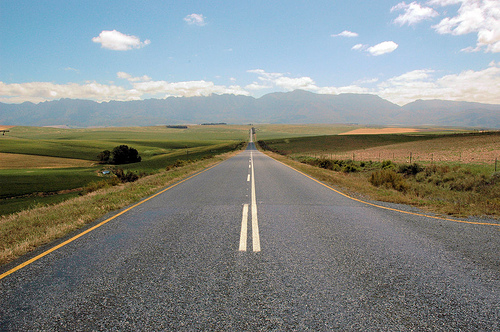
\includegraphics[width=0.5\textwidth]{photos/roadby_cornstaruk_flickr.jpg}
\end{center}
\end{Investigation}



\section{Versnelling}
\Definition{Gemiddelde versnelling} {Gemiddelde versnelling is die verandering in gemiddelde snelheid gedeel deur die tyd wat geneem is.\\
Simbool: $\vec{a}_{av}$\hspace{2cm} S.I. Eenhede: $\text{m} \cdot \text{s}^{-2}$ } 

Versnelling is 'n mate van hoe vinnig  die snelheid van 'n voorwerp oor tyd verander. As ons 'n verander in snelheid ($\Delta \vec{v}$) het, oor 'n tydsinterval ($\Delta t$), dan word die gemiddelde versnelling ($\vec{a}_{av}$) gedefini\"eer as:

\begin{equation*}
    \text{gemiddelde versnelling (in m} \cdot {\text{s}}^{-2}\text{)} =\frac{\text{verandering in snelheid (in m} \cdot {\text{s}}^{-1}\text{)}}{\text{verandering in tyd (in s)}}
      \end{equation*}
        
    \begin{equation*}
    \vec{a}_{av}=\frac{\Delta \vec{v}}{\Delta t}
      \end{equation*}

Ons werk net met probleme wat konstante versnelling behels. Dit beteken dat die gemiddelde versnelling en die oombliklike versnelling diselfde is. Om dinge makliker te maak sal ons net praat van versnelling en nie ``gemiddeld'' of ``oombliklik'' nie. Dit word as $\vec{a}$ voorgstel. Ons het ook die grootte van die versnelling. Dit is:
\begin{equation*}
    a=\frac{\Delta \vec{v}}{\Delta t}
\end{equation*}

Versnelling is 'nm vektor. Versnelling s\^e niks van die beweging nie maar net hoe vinnig die bewegin verander. Dit is nie moontlik om te s\^e hoe vinnig 'n voorwerp beweeg of in watter rigting dit beweeg van die snelheid aleenlik nie.\par

Soos snelheid, kan versnelling ook positief of negatief wees. Wanneer die teken van die versnelling en die snelheid dieselfde is, beweeg die voorwerp al hoe vinniger. As die beide die versnelling en snelheid positief is, beweeg die voorwerp al hoe vinniger in die positiewe rigting. Netso, as beide negatief is beweeg die voorwerp die al hoe vinniger in die negatiewe rigting.      

\Tip{Vermy die woord \textsl{vertraging} as jy na 'n negatiewe versnelling verwys. Dit beteken gewoonlik \textsl{vermindering in spoed} maar dit is moontlik vir 'n voorwerp om spoed te verminder met beide 'n positiewe of negatiewe versnelling, want die teken van die snelheid moet ook in ag geneem word om vas te stel of 'n voorwerp spoed verminder of nie.}

Ons kan dit sien in die volgende diagram:
\begin{figure}[H]
 \begin{center}
  \begin{pspicture}(-5,-1)(5,3)
\rput(-3,0){
\pspolygon(0,0)(0,1)(1,1)(1,0)(0,0)
\psline{->}(0.3,1.1)(0.9,1.1)
\rput[tl](0.3,1.5){$\vec{v}$}
\psline{->}(0.5,0.5)(1.5,0.5)
\rput[tr](1.5,0.3){$\vec{a}$}
\rput(.8,-.3){beweeg vinniger}}
\rput(-0.5,0){
\pspolygon(0,0)(0,1)(1,1)(1,0)(0,0)
\psline{<-}(0.3,1.1)(0.9,1.1)
\rput[tl](0.3,1.5){$\vec{v}$}
\psline{->}(0.5,0.5)(1.5,0.5)
\rput[tr](1.5,0.3){$\vec{a}$}
\rput(.8,-.3){beweeg stadiger}
}
\rput(3,0){
\pspolygon(0,0)(0,1)(1,1)(1,0)(0,0)
\psline{<-}(0.3,1.1)(0.9,1.1)
\rput[tl](0.3,1.5){$\vec{v}$}
\psline{->}(0.5,0.5)(-0.5,0.5)
\rput[tr](-.5,0.3){$\vec{a}$}
\rput(.8,-.3){beweeg vinniger}
\rput(.8,-.6){negatiewe versnelling}}
  \end{pspicture}
 \end{center}
\end{figure}

As snelheid positief is en versnelling is negatief, dan sal die voorwerp se spoed verminder. Op dieselfde manier, as die snelheid negatief en die versnelling positief is, sal die voorwerp se spoed verminder. Dit word in die volgende voorbeeld illustreer.

\begin{wex}{Versnelling}{'n Kar versnel eenvormig van 'n aanvanklike snelheid van 2 m$\cdot$s$^{-1}$ tot 'n finale snelheid van 10 m$\cdot$s$^1$ in 8 sekondes. Dit verminder dan spoed teen 'n egalige tempo tot 'n finale snelheid van 4 m$\cdot$s$^{-1}$ in 6 sekondes. Bereken die versnelling van die kar gedurende die eerste 8 sekondes en gedurende die laaste 6 sekondes.}
{
\westep{Kies 'n verwysingsraamwerk}
Ons kies die punt waar die kar sy versnelling begin as die oorsproing en die rigting waarin hy alreeds beweeg as die positiewe rigting.
\westep{Identifiseer watter inligting gegee is en wat gevra word}
Beskou die beweging van die kar in twee dele: die eerste 8 sekondes en die laaste 6 sekondes.\\

\begin{minipage}{0.5\textwidth}
\center{Vir die eerste 8 sekondes:}
\begin{eqnarray*}
\vec{v}_i &=& 2~\text{m}\cdot \text{s}^{-1}\\
\vec{v}_f &=& 10~\text{m}\cdot \text{s}^{-1}\\
t_i &=& 0~\text{s}\\
t_f &=& 8~\text{s}
\end{eqnarray*}
\end{minipage}
\begin{minipage}{0.5\textwidth}
\center{Vir die laaste 6 sekondes:}
\begin{eqnarray*}
\vec{v}_i &=& 10~\text{m}\cdot \text{s}^{-1}\\
\vec{v}_f &=& 4~\text{m}\cdot \text{s}^{-1}\\
t_i &=& 8~\text{s}\\
t_f &=& 14~\text{s}
\end{eqnarray*}

\end{minipage}\\

\westep{Bereken die versnelling}
\begin{minipage}[t]{0.5\textwidth}
\center{Vir die eerste 8 sekondes:}
\begin{eqnarray*}
a &=& \frac{\Delta v}{\Delta t}\\
&=& \frac{10\textrm{ \text{m}\cdot \text{s}^{-1}} - 2\textrm{ \text{m}\cdot \text{s}^{-1}}}{8\textrm{ s} - 0\textrm{ s}}\\
&=& 1~\text{m}\cdot \text{s}^{-2}
\end{eqnarray*}

\end{minipage}
\begin{minipage}[t]{0.5\textwidth}
\center{Vir die laaste 6 sekondes:}
\begin{eqnarray*}
a &=& \frac{\Delta v}{\Delta t}\\
&=& \frac{4\textrm{ \text{m}\cdot \text{s}^{-1}} - 10\textrm{ \text{m}\cdot \text{s}^{-1}}}{14\textrm{ s} - 8\textrm{ s}}\\
&=& -1~\text{m}\cdot \text{s}^{-2}
\end{eqnarray*}

\end{minipage}\\
Gedurende die eerste 8 sekondes het die kar 'n positiewe versnelling. Die kar se snelheid is ook positief en dus vermeerder die kar se spoed.\par
Gedurende die volgende 6 sekondes het die kar 'n negatiewe versnelling maar 'n positiewe snelheid. Dit beteken die kar verminder spoed.
}
\end{wex}


\begin{exercises}{Versnelling}
      
\noindent
\begin{enumerate}[noitemsep, label=\textbf{\arabic*}. ] 
    \item 'n Atleet versnel eenvormig van 'n aanvanklike snelheid van 0 m$\ensuremath{\cdot}$s${}^{-1}$ tot 'n finale snelheid van 4 m$\ensuremath{\cdot}$s${}^{-1}$ in 2 sekondes. Bereken sy versnelling. Maak die rigting waarin die atleet hardloop positief.    
    \item \n Bus versnel eenvormig van 'n aanvanklike snelheid van 15 m$\ensuremath{\cdot}$s${}^{-1}$ tot 'n finale snelheid van 7~m$\ensuremath{\cdot}$s${}^{-1}$ in 4 sekondes. Bereken die versnelling van die bus. Maak die rigting waarin die bus beweeg positief.

    \item 'n Vliegtuig versnel eenvormig van 'n snelheid van 200 m$\ensuremath{\cdot}$s${}^{-1}$ tot 'n snelheid van100 m$\ensuremath{\cdot}$s${}^{-1}$in 10 sekondes. Dit versnel dan eenvormig tot 'n finale snelheid van 240 m$\ensuremath{\cdot}$s${}^{-1}$in 20 sekondes. Maak die rigting waarin die vliegtuig beweeg positief.
 
    \begin{enumerate}[noitemsep, label=\textbf{\alph*}. ] 
            \item Bereken die versnelling van die vliegtuig gedurende die eerste 10 sekondes.
            \item Bereken die versnelling van die vliegtuig gedurende die volgende 14 sekondes.
    \end{enumerate}
\end{enumerate}
\par \raisebox{-5 pt}{
\includegraphics[width=0.5cm]{col11305.imgs/summary_www.png}} Vind antwoorde met die volgende kortkodes:
\par \begin{tabular}[h]{cccccc}
(1.) l1k  &  (2.) l10  &  (3.) l18  & \end{tabular}
\end{exercises}

Die volgende video gee 'n opsomming van afstand, snelheid en versnelling. Neem kennis dat daar 'n ander konvensie vir eenhede gebruik word in hierdie video. Jy behoort nie hierdie video se konvensie te gebruik nie vir fisika nie.
	\begin{figure}[H] % horizontal\label{m38794*motion-1}
    \textnormal{Khan academy video oor beweging - 1} \nopagebreak
  \label{m38794*yt-media1}\label{m38794*yt-video1}
            \raisebox{-5 pt}{ 
\includegraphics[width=0.5cm]{col11305.imgs/summary_www.png}} { (Video:  P10101 )}
 \end{figure}       \par 
%NTS CAPS says that instantaneous speed and velocity must only be covered now and not be covered where they currently are
\nopagebreak


\section{Oombliklike snelheid en spoed}


\begin{minipage}{.5\textwidth}
\begin{center}
\textbf{Naellopers spring weg}\\
\includegraphics[width=.8\textwidth]{photos/sprintersstarting_wwarby_flickr.jpg}\\
\textbf{Einde van resies}\\
\includegraphics[width=.8\textwidth]{photos/sprintersending_wwarby_flickr.jpg}\\
\textit{Fotos deur wwarby op Flickr.}
\end{center}
\end{minipage}
\begin{minipage}{.5\textwidth}

Ons het gekyk na die gemiddelde snelheid en spoed maar soms wil ons meer presies weet wat gebeur tussen die aanvanklike en finale tye in 'n probleem.

Oombliklike snelheid is die snelheid op 'n spesifieke tyd. Dit kan anders wees as die gemiddelde snelheid as die snelheid nie konstant is nie.

Kyk na die fotos van die naellopers in 'n wedloop. Hul snelheid by die wegspring is anders as aan die einde van die resies. Hulle gemiddelde snelheid vir die resies verander nie maar hulle oombklilike snelheid, soos vasgevang in die fotos op 'n sekere tyd, verander wel. Die snelheid van die naelloper toe die die foto geneem is, is sy oombliklike snelheid.

\end{minipage}

\Tip{'n Oomblik in tyd is anders as die tyd geneem of 'n tydsinterval. Dit is dus handig om die simbool $t$ te gebruik vir 'n oomblik in tyd (byvoorbeeld gedurende die 4$^\text{e}$ sekonde) en die simbool $\Delta t$ vir 'n tydsinterval (byvoorbeeld die eerste 5 sekondes van die beweging).}\\


\Definition{Oombliklike snelheid}{Oombliklike snelheid is die verandering in posisie oor die verandering in 'n bye kort tydsinterval. ($\Delta t \approx 0$). \\
Simbool: $\vec{v}$\hspace{2cm} S.I. Eenhede: $\text{m}\cdot \text{s}^{-1}$} 

\Definition{Oombliklike spoed}{Oombliklike spoed is die grootte van oombliklike snelheid.\\
Symbol: $v$\hspace{2cm} S.I. Units: $\text{m}\cdot \text{s}^{-1}$} 

Oombliklike snelheid is 'n vektor. Oombliklike spoed is die grootte van oombliklike snelheid. Die het dieselfde waarde maar het nie 'n rigting nie en is dus nie 'n vektor nie.


\section{Beskrywing van beweging}
%NTS this section needs a formal project on acceleration

Die doel van hierdie hoofstuk is om beweging te beskryf en nou dat ons die definisies van verplasing, afstand, snelheid, spoed en versnelling verstaan, is ons gereed om hierdie idees te gebruik om te beskryf hoe 'n voorwerp of persoon beweeg. Ons sal na drie maniere  om beweging te beskryf kyk:\par 
\begin{enumerate}[noitemsep, label=\textbf{\arabic*}. ] 
    \item woorde
    \item diagramme
    \item grafieke
\end{enumerate}
Hierdie metodes sal in die volgende seksie beskryf word. \par 
Ons sal drie soorte beweging beskou: wanneer 'n voorwerp nie beweeg nie (stilstaande voorwerp), wanneer 'n voorwerp teen 'n konstante snelheid bweeg (eenvormige beweging) en wanneer 'n voorwerp teen 'n konstante tempo versnel (beweging teen konstante versnelling).\par 

\subsection*{Stilstaande Voorwerpe}
\nopagebreak
Die eenvoudigste bewegin wat ons te\"e kom is di\'e van 'n stilstaande voorwerp. 'n Stilstaande voorwerp beweeg nie en sy posisie verander nie.

\begin{minipage}{.5\textwidth}
Beskou die volgende voorbeeld. Vivian wag vir 'n taxi. Sy staan twee meter vanaf 'n stopstraat by $t=0~\text{s}$. Na een minuut, by $t=60~\text{s}$, staan sy nog steeds 2 meter van die stopstraat en na twee minute, by $t=120~\text{s}$ staan sy ook  2 meter vanaf die stopstraat. Haar posisie het nie verander nie. Haar verplasing is nul (want haar posisie is nog dieselfde), haar snelheid is nul want haar verplasing is nul en haar versnelling is ook nul (want haar snelheid het nie verander nie ).

Ons kan nou grafieke trek van posisie teen tyd ($\vec{x}$ vs. $t$), snelheid teen tyd ($\vec{v}$ vs. $t$) en versnelling teen tyd ($\vec{a}$ vs. $t$) vir 'n stilstaande voorwerp. Die grafieke word hieronder gewys.
\end{minipage}
\begin{minipage}{.5\textwidth}
\begin{center}
 \textbf{Vivian staan by 'n stopstraat.}\\
%\includegraphics[width=.8\textwidth]{photos/stopstreet_by_CarolynColes_Flickr.jpg}\\
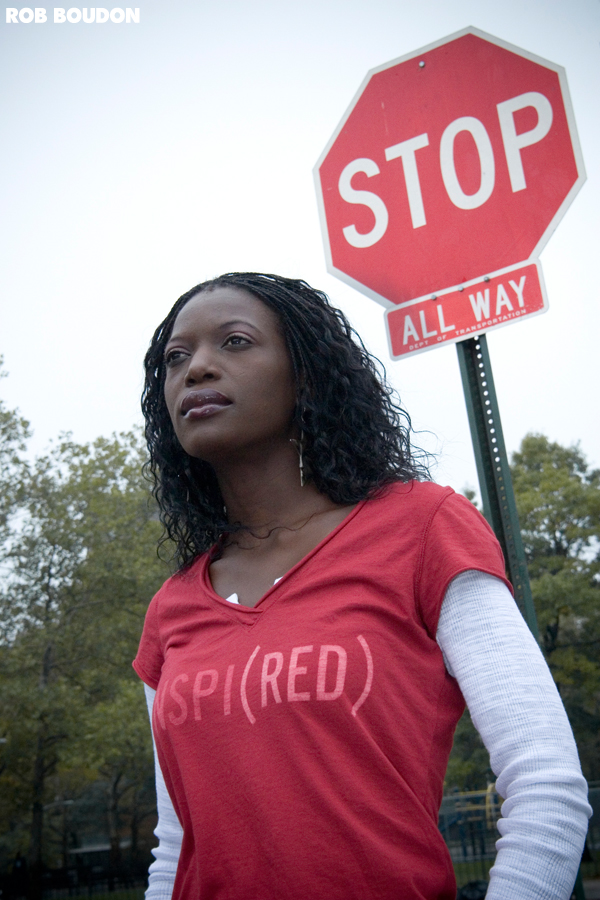
\includegraphics[width=.8\textwidth]{photos/stopstreet_by_RobBoudon_Flickr.jpg}\\
\textit{Foto deur Rob Boudon op Flickr}
\end{center}
\end{minipage}



\begin{center}
\scalebox{1} % Change this value to rescale the drawing.
{
\begin{pspicture}(0,-2.3034375)(15.0207815,2.3034375)

\rput(9.671615,2.3734374){   }
\psline[]{->}(0.79578125,-1.1865625)(0.79578125,1.8134375)
\psline[]{->}(0.79578125,-1.1865625)(3.7957811,-1.1865625)
\psline[]{->}(5.795781,-1.1865625)(5.795781,1.8134375)
\psline[]{->}(5.795781,-1.1865625)(8.795781,-1.1865625)
\psline[]{->}(10.795781,-1.1865625)(10.795781,1.8134375)
\psline[]{->}(10.795781,-1.1865625)(13.795781,-1.1865625)
\psline[linewidth=0.09cm](10.795781,-1.1865625)(12.795781,-1.1865625)
\psline[linewidth=0.09cm](5.795781,-1.1865625)(7.795781,-1.1865625)
\psline[linewidth=0.09cm](0.79578125,0.8134375)(2.7957811,0.8134375)

\rput(1.7615625,-1.4765625){60}

\rput(2.8382812,-1.4765625){120}

\rput(0.574375,0.8234375){2}

\rput(0.54265624,-0.1765625){1}

\rput(0.5728125,-1.2765625){0}

\rput(7.838281,-1.4765625){120}

\rput(12.738281,-1.4765625){120}
\psline[](1.7957813,-1.0865625)(1.7957813,-1.1865625)
\psline[](2.7957811,-1.0865625)(2.7957811,-1.1865625)
\psline[](6.795781,-1.0865625)(6.795781,-1.1865625)
\psline[](7.795781,-1.0865625)(7.795781,-1.1865625)
\psline[](11.795781,-1.0865625)(11.795781,-1.1865625)
\psline[](12.795781,-1.0865625)(12.795781,-1.1865625)
\psline[](0.69578123,-0.1865625)(0.8957813,-0.1865625)
\psline[](0.69578123,0.8134375)(0.79578125,0.8134375)

\rput(4.4365625,-1.1765625){tyd(s)}

\rput(9.436563,-1.1765625){tyd (s)}

\rput(14.436563,-1.1765625){tyd (s)}

\rput{-270.0}(0.571875,0.2365625){\rput(0.16890626,0.4234375){posisie $x$ (m)}}

\rput{-270.0}(5.9035935,-5.0960937){\rput(5.496719,0.4234375){snelheid $v$ (\ms)}}

\rput{-270.0}(10.958906,-10.150469){\rput(10.541875,0.4234375){versnelling $a$ (m$\cdot$s$^{-2}$)}}

\rput(5.6728125,-1.2765625){0}

\rput(10.672812,-1.2765625){0}

\rput(6.7615623,-1.4765625){60}

\rput(11.761562,-1.4765625){60}

\rput(1.9809375,-2.0765624){(a)}

\rput(6.9909377,-2.0765624){(b)}

\rput(11.980938,-2.0765624){(c)}
\psline[](2.7957811,0.8134375)(2.7957811,-1.0865625)
\end{pspicture} 
}
\caption{Grafieke vir 'n stilstaande voorwerp (a) posisie teen tyd (b) snelheid teen tyd (c) versnelling teen tyd.}
\label{fig:pr:stationary}
\end{center}

Vivian se posisie is 2~meter vanaf die stopstraat as die stopteken as die verwysingspunt geneem word. Haar posisie bly 2~meter vir 120~sekondes. Die grafiek is 'n horisontale lyn by $2 \text{ m}$. Die snelheid en versnelling grafieke word ook gewys. Hulle is albei horisontale lyne op die $x$-as. Omdat haar posisie nie verander nie, is haar snelheid $0~\text{m}\ensuremath{\cdot}\text{s}{}^{-1}$ en omdat haar snelheid nie verander nie, is haar versnelling $0~\text{m}\ensuremath{\cdot}\text{s}{}^{-2}$.\par 


\par
\Definition{Gradi\"ent} {Die gradi\"ent, $m$, van 'n lyn kan bereken word deur die verandering in die $y$ waarde (afhanklike veranderlike) te deel deur die verandering in die $x$ waarde (onafhanklike veranderlike) $$m = \frac{\Delta y}{\Delta x}$$ \par  } 

Omdat ons weet dat snelheid die tempo van verandering van posisie is, kan ons die waarde van die snelheid teen tyd grafiek bevesting deur die gradi\"ent van die $\vec{x}$ vs. $t$ grafiek te bereken.\par 

\Tip{Die gradi\"ent van 'n posisie teen tyd grafiek gee die snelheid.}
	\par
As ons die gradi\"ent van die $\vec{x}$~vs.~$t$ grafiek van 'n stilstaande voorwerp bereken, kry ons:\par 
        \label{m38795*id69332}\nopagebreak\noindent{}
    \begin{align*}
	v &= \frac{\Delta \vec{x}}{\Delta t}\\
	&= \frac{\vec{x}_{f}-\vec{x}_{i}}{{t}_{f}-{t}_{i}}\\
	&= \frac{2~\text{m}-2~\text{m}}{120~\text{s}-60~\text{s}} \left(\text{aanvanklike\; posisie}=\text{finale\; posisie}\right)\\ 
	&= 0~\text{m}\ensuremath{\cdot}{\text{s}}^{-1}  \left(\text{gedurende\; die \; tyd\; wat\; Vivian\; stilstaande\; is}~\right) \\
      \end{align*}
Op 'n soortgelyke manier kan ons die waarde van die versnelling bevestig deur die gradi\"ent van die snelheid teen tyd grafiek te bereken.\par 

\Tip{Die gradi\"ent van 'n snelheid teen tyd grafiek is die versnelling.}
	\par
As ons die gradi\"ent van die $\vec{v}$ vs. $t$ grafiek van 'n stilstaande voorwerp bereken, kry ons:\par 
        \label{m38795*id69594}\nopagebreak\noindent{}
          
    \begin{align*}
    a &= \frac{\Delta v}{\Delta t}\hfill \\ 
    &= \frac{\vec{v}_{f}-\vec{v}_{i}}{{t}_{f}-{t}_{i}}\hfill \\ 
    &= \frac{0~\text{m}\cdot\text{s}^{-1}-0~\text{m}\cdot\text{s}^{-1}}{120~\text{s}-60~\text{s}}\\ 
    &= 0~\text{m}\cdot\text{s}^{-2}
      \end{align*}

Daarbenewens, omdat die snelheid teen tyd grafiek verwant is aan die posisie teen tyd grafiek, kan ons die oppervlak onder die snelheid teen tyd grafiek gebruik om die verplasing van 'n voorwerp te bereken.\par 

\Tip{Die oppervlak onder die snelheid teen tyd grafiek gee die verplasing.}
	\par

Die verplasing van die voorwerp word gegee deur die oppervlak onder die grafiek, wat $0~\text{m}$ is. Dit is voor die hand liggend want die voorwerp beweeg nie.\par 


\subsection*{Beweging teen konstante snelheid}
\nopagebreak
Beweging teen 'n konstante snelheid of \textsl{eenvormige beweging} beteken dat die posisie van 'n voorwerp teen 'n konstante tempo verander.\par 
Neem aan dat dit Vivian $100~\text{s}$ vat om die $100~\text{m}$ na die taxi-stop af te l\^e. As ons aanneem dat Vivian se huis die oorsprong is, dan is Vivian se snelheid:\par 
        \label{m38795*id69850}\nopagebreak\noindent{}
          
    \begin{align*}
    	v&= \frac{\Delta \vec{x}}{\Delta t}\hfill \\ 
	&= \frac{{x}_{f}-{x}_{i}}{{t}_{f}-{t}_{i}}\hfill \\ 
	&= \frac{100~\text{m}-0~\text{m}}{100~\text{s}-0~\text{s}}\\ 
	 &= 1~\text{m}\cdot{\text{s}}^{-1}
      \end{align*}
Vivian se snelheid is 1 m$\ensuremath{\cdot}$s${}^{-1}$. Dit beteken dat sy $1~\text{m}$ gestap het in die eerste sekonde, nog 'n meter in die tweede sekonde, en nog 'n meter in die derde sekonde ensovoorts. Byvoorbeeld, na $50~\text{s}$ sal sy $50~\text{m}$ van die huis af wees.from home. Haar posisie vermeerder met $1~\text{m}$ elke $1~\text{s}$. 'n Diagram van Vivian se posisie word hieronder gewys:\par 

\begin{center}
\scalebox{1} % Change this value to rescale the drawing.
{
\begin{pspicture}(0,-1.57375)(9.02,1.53375)
\psline[]{->}(2.0,-0.46625)(9.0,-0.46625)
\psframe[linewidth=0.04,dimen=outer](2.0,0.53375)(0.0,-0.46625)
\pstriangle[linewidth=0.04,dimen=outer](1.0,0.53375)(2.0,1.0)
\psframe[linewidth=0.04,dimen=outer](1.2,0.23375)(0.8,-0.46625)
\psframe[linewidth=0.04,dimen=outer](1.8,0.23375)(1.4,-0.06625)
\psframe[linewidth=0.04,dimen=outer](0.6,0.23375)(0.2,-0.06625)
\psellipse[linewidth=0.04,dimen=outer](2.15,0.53375)(0.15,0.2)
\psline[](2.1,0.33375)(2.1,0.33375)
\psline[linewidth=0.051999997cm](2.14,0.37375)(2.14,-0.02625)
\psline[](2.14,-0.02625)(2.24,-0.24625)
\psline[](2.24,-0.24625)(2.2,-0.42625)
\psline[](2.2,-0.42625)(2.3,-0.42625)
\psline[](2.12,-0.00625)(2.1,-0.26625)
\psline[](2.1,-0.26625)(2.02,-0.42625)
\psline[](2.02,-0.42625)(2.12,-0.42625)
\psline[](2.12,0.27375)(2.04,0.03375)
\psline[](2.04,0.03375)(2.22,0.15375)
\psline[](2.12,0.21375)(2.24,-0.02625)
\psline[](2.24,-0.02625)(2.32,0.03375)
\psdots[dotsize=0.04](2.2,0.59375)
\pscustom[linewidth=0.04]
{
\newpath
\moveto(2.12,0.51375)
\lineto(2.17,0.47375)
\curveto(2.195,0.45375)(2.225,0.43875)(2.24,0.45375)
}
\pscustom[linewidth=0.04]
{
\newpath
\moveto(2.24,0.69375)
\lineto(2.19,0.70375)
\curveto(2.165,0.70875)(2.12,0.70875)(2.1,0.70375)
\curveto(2.08,0.69875)(2.05,0.67875)(2.04,0.66375)
\curveto(2.03,0.64875)(2.015,0.62875)(2.0,0.61375)
}
\pscustom[linewidth=0.04]
{
\newpath
\moveto(2.0,0.61375)
\lineto(2.03,0.64375)
\curveto(2.045,0.65875)(2.08,0.67875)(2.1,0.68375)
\curveto(2.12,0.68875)(2.165,0.69375)(2.19,0.69375)
\curveto(2.215,0.69375)(2.245,0.68375)(2.26,0.65375)
}
\pscustom[linewidth=0.04]
{
\newpath
\moveto(2.14,0.71375)
\lineto(2.1,0.67375)
\curveto(2.08,0.65375)(2.055,0.61875)(2.04,0.57375)
}

\rput[l](8,-1.05625){$x$ = 100 m}

\rput[l](2,-0.73625){t = 0 s}

\rput[l](5,-0.73625){t = 50 s}

\rput[l](8,-0.73625){t = 100 s}

\rput[l](5,-1.05625){$x$ = 50 m}

\rput[l](2,-1.05625){$x$ = 0 m}
\psline[](5.0,1.07375)(5.0,-0.44625)
\psline[](7.98,1.05375)(7.98,-0.46625)
\psellipse[linewidth=0.04,dimen=outer](5.17,0.51375)(0.15,0.2)
\psline[](5.12,0.31375)(5.12,0.31375)
\psline[linewidth=0.051999997cm](5.16,0.35375)(5.16,-0.04625)
\psline[](5.16,-0.04625)(5.26,-0.26625)
\psline[](5.26,-0.26625)(5.22,-0.44625)
\psline[](5.14,-0.02625)(5.12,-0.28625)
\psline[](5.12,-0.28625)(5.04,-0.44625)
\psline[](5.14,0.25375)(5.06,0.01375)
\psline[](5.06,0.01375)(5.24,0.13375)
\psline[](5.14,0.19375)(5.26,-0.04625)
\psline[](5.26,-0.04625)(5.34,0.01375)
\psdots[dotsize=0.04](5.22,0.57375)
\pscustom[linewidth=0.04]
{
\newpath
\moveto(5.14,0.49375)
\lineto(5.19,0.45375)
\curveto(5.215,0.43375)(5.245,0.41875)(5.26,0.43375)
}
\pscustom[linewidth=0.04]
{
\newpath
\moveto(5.26,0.67375)
\lineto(5.21,0.68375)
\curveto(5.185,0.68875)(5.14,0.68875)(5.12,0.68375)
\curveto(5.1,0.67875)(5.07,0.65875)(5.06,0.64375)
\curveto(5.05,0.62875)(5.035,0.60875)(5.02,0.59375)
}
\pscustom[linewidth=0.04]
{
\newpath
\moveto(5.02,0.59375)
\lineto(5.05,0.62375)
\curveto(5.065,0.63875)(5.1,0.65875)(5.12,0.66375)
\curveto(5.14,0.66875)(5.185,0.67375)(5.21,0.67375)
\curveto(5.235,0.67375)(5.265,0.66375)(5.28,0.63375)
}
\pscustom[linewidth=0.04]
{
\newpath
\moveto(5.16,0.69375)
\lineto(5.12,0.65375)
\curveto(5.1,0.63375)(5.075,0.59875)(5.06,0.55375)
}
\psellipse[linewidth=0.04,dimen=outer](8.13,0.55375)(0.15,0.2)
\psline[](8.08,0.35375)(8.08,0.35375)
\psline[linewidth=0.051999997cm](8.12,0.39375)(8.12,-0.00625)
\psline[](8.1,0.01375)(8.08,-0.24625)
\psline[](8.1,0.29375)(8.02,0.05375)
\psline[](8.02,0.05375)(8.2,0.17375)
\psline[](8.1,0.23375)(8.22,-0.00625)
\psline[](8.22,-0.00625)(8.3,0.05375)
\psdots[dotsize=0.04](8.18,0.61375)
\pscustom[linewidth=0.04]
{
\newpath
\moveto(8.1,0.53375)
\lineto(8.15,0.49375)
\curveto(8.175,0.47375)(8.205,0.45875)(8.22,0.47375)
}
\pscustom[linewidth=0.04]
{
\newpath
\moveto(8.22,0.71375)
\lineto(8.17,0.72375)
\curveto(8.145,0.72875)(8.1,0.72875)(8.08,0.72375)
\curveto(8.06,0.71875)(8.03,0.69875)(8.02,0.68375)
\curveto(8.01,0.66875)(7.995,0.64875)(7.98,0.63375)
}
\pscustom[linewidth=0.04]
{
\newpath
\moveto(7.98,0.63375)
\lineto(8.01,0.66375)
\curveto(8.025,0.67875)(8.06,0.69875)(8.08,0.70375)
\curveto(8.1,0.70875)(8.145,0.71375)(8.17,0.71375)
\curveto(8.195,0.71375)(8.225,0.70375)(8.24,0.67375)
}
\pscustom[linewidth=0.04]
{
\newpath
\moveto(8.12,0.73375)
\lineto(8.08,0.69375)
\curveto(8.06,0.67375)(8.035,0.63875)(8.02,0.59375)
}
\psline[](8.14,-0.44625)(8.22,-0.44625)
\psline[](8.02,-0.44625)(8.1,-0.44625)
\psline[](8.12,-0.00625)(8.22,-0.22625)
\psline[](8.08,-0.22625)(8.02,-0.44625)
\psline[](8.22,-0.20625)(8.14,-0.44625)
\psline[](5.02,-0.42625)(5.12,-0.42625)
\psline[](5.2,-0.42625)(5.28,-0.42625)

\rput[l](5,-1.37625){$v$ = 1\text{m}\cdot \text{s}^{-1}}

\rput[l](8,-1.39625){$v$ = 1\text{m}\cdot \text{s}^{-1}}
\end{pspicture} 
}
\end{center}
\caption{Diagram van Vivian se beweging teen 'n konstante snelheid van 1 \text{m}\cdot \text{s}^{-1} wys.}
\label{fig:pr:diagram:uniform}

Ons kan nou grafieke van posisie teen tyd ($\vec{x}$ vs. $t$), snelheid teen tyd ($\vec{v}$ vs. $t$) en versnelling teen tyd ($\vec{a}$ vs. $t$) teken vir Vivian se beweging teen 'n konstante snelheid. Die grafieke word hier gewys:
\begin{center}
\scalebox{1} % Change this value to rescale the drawing.
{
\begin{pspicture}(0,-2.3034375)(15.220781,2.3034375)
\definecolor{color1158b}{rgb}{0.8,0.8,0.8}

\rput(9.871614,2.3734374){   }
\psline[]{->}(0.99578124,-1.1865625)(0.99578124,1.8134375)
\psline[]{->}(0.99578124,-1.1865625)(3.9957812,-1.1865625)
\psline[]{->}(5.9957814,-1.1865625)(5.9957814,1.8134375)
\psline[]{->}(5.9957814,-1.1865625)(8.995781,-1.1865625)
\psline[]{->}(10.995781,-1.1865625)(10.995781,1.8134375)
\psline[]{->}(10.995781,-1.1865625)(13.995781,-1.1865625)
\psline[linewidth=0.09cm](10.995781,-1.1865625)(12.995781,-1.1865625)
\psline[linewidth=0.09cm](5.9957814,-0.1865625)(7.9957814,-0.1865625)
\psline[linewidth=0.09cm](0.99578124,-1.1865625)(2.9957812,0.8134375)

\rput(1.9607812,-1.4765625){50}

\rput(3.0382812,-1.4765625){100}

\rput(0.53828126,0.8234375){100}

\rput(0.66078126,-0.1765625){50}

\rput(0.7728125,-1.2765625){0}

\rput(8.038281,-1.4765625){100}

\rput(12.938281,-1.4765625){100}
\psline[](1.9957813,-1.0865625)(1.9957813,-1.1865625)
\psline[](2.9957812,-1.0865625)(2.9957812,-1.1865625)
\psline[](6.9957814,-1.0865625)(6.9957814,-1.1865625)
\psline[](7.9957814,-1.0865625)(7.9957814,-1.1865625)
\psline[](11.995781,-1.0865625)(11.995781,-1.1865625)
\psline[](12.995781,-1.0865625)(12.995781,-1.1865625)
\psline[](0.8957813,-0.1865625)(1.0957812,-0.1865625)
\psline[](0.8957813,0.8134375)(0.99578124,0.8134375)

\rput(4.6365623,-1.1765625){tyd (s)}

\rput(9.636562,-1.1765625){tyd (s)}

\rput(14.636562,-1.1765625){tyd (s)}

\rput{-270.0}(0.571875,0.2365625){\rput(0.16890626,0.4234375){posisie $x$ (m)}}

\rput{-270.0}(5.8035936,-4.9960938){\rput(5.396719,0.4234375){snelheid $v$ (\ms)}}

\rput{-270.0}(11.0,-10.350469){\rput(10.741875,0.4234375){versnelling $a$ (m$\cdot$s$^{-2}$)}}

\rput(5.8728123,-1.2765625){0}

\rput(10.872812,-1.2765625){0}

\rput(6.960781,-1.4765625){50}

\rput(11.960781,-1.4765625){50}

\rput(2.1809375,-2.0765624){(a)}

\rput(7.1909375,-2.0765624){(b)}

\rput(12.180938,-2.0765624){(c)}
\psline[](2.9957812,0.8134375)(2.9957812,-1.0865625)

\rput(5.742656,-0.1765625){1}
\psline[](5.895781,-0.1865625)(6.0957813,-0.1865625)
\psline[](2.8957813,0.8134375)(0.99578124,0.8134375)
\psline[](7.9957814,-0.1865625)(7.9957814,-1.1865625)
\psframe[linewidth=0.02,linecolor=color1158b,dimen=outer,fillstyle=solid,fillcolor=color1158b](7.9757814,-0.2265625)(6.0157814,-1.1465625)
\psline[linewidth=0.03cm,](2.5757813,0.3534375)(2.5757813,-0.5865625)
\psline[linewidth=0.03cm,](2.5757813,-0.5865625)(1.6357813,-0.5865625)
\rput[l](2.7,-0.1365625){$\Delta$x}
\rput(2.2054687,-0.7315625){\footnotesize $\Delta$t}
\end{pspicture} 
}
\caption{Grafieke vir konstante snelheid (a) posisie teen tyd (b) snelheid teen tyd (c) versnelling teen tyd. Die oppervlak van die ingekleurde deel in die $v$ vs. $t$ grafiek stem ooreen met die voorwerp se verplasing.}
\label{fig:pr:uniform}
\end{center}

In die aand loop Vivian $100~\text{m}$ van die busstop to by haar huis in $100~\text{s}$. Ons neem aan Vivian se huis is die oorsprong. Die volgende grafieke kan geteken word om die beweging te beskryf.\par 
\begin{center}
\scalebox{1} % Change this value to rescale the drawing.
{
\begin{pspicture}(0,-2.3034375)(15.220781,2.3034375)
\definecolor{color1158b}{rgb}{0.8,0.8,0.8}

\rput(9.871614,2.3734374){   }
\psline[]{->}(0.99578124,-1.1865625)(0.99578124,1.8134375)
\psline[]{->}(0.99578124,-1.1865625)(3.9957812,-1.1865625)
\psline[]{<->}(6.0110865,1.8133594)(5.980476,-1.1864845)
\psline[]{->}(5.9957814,0.8134375)(8.995781,0.8134375)
\psline[]{->}(10.995781,-1.1865625)(10.995781,1.8134375)
\psline[]{->}(10.995781,-1.1865625)(13.995781,-1.1865625)
\psline[linewidth=0.09cm](10.995781,-1.1865625)(12.995781,-1.1865625)
\psline[linewidth=0.09cm](5.9957814,-0.1865625)(7.9957814,-0.1865625)
\psline[linewidth=0.09cm](0.97578126,0.8134375)(2.9957812,-1.1865625)

\rput(1.9607812,-1.4765625){50}

\rput(3.0382812,-1.4765625){100}

\rput(0.53828126,0.8234375){100}

\rput(0.66078126,-0.1765625){50}

\rput(0.7728125,-1.2765625){0}

\rput(7.938281,1.0234375){100}

\rput(12.938281,-1.4765625){100}
\psline[](1.9957813,-1.0865625)(1.9957813,-1.1865625)
\psline[](2.9957812,-1.0865625)(2.9957812,-1.1865625)
\psline[](6.9957814,0.9134375)(6.9957814,0.8134375)
\psline[](7.9957814,0.9134375)(7.9957814,0.8134375)
\psline[](11.995781,-1.0865625)(11.995781,-1.1865625)
\psline[](12.995781,-1.0865625)(12.995781,-1.1865625)
\psline[](0.8957813,-0.1865625)(1.0957812,-0.1865625)
\psline[](0.8957813,0.8134375)(0.99578124,0.8134375)

\rput(4.6365623,-1.1765625){tyd (s)}

\rput(9.536563,0.8234375){tyd (s)}

\rput(14.636562,-1.1765625){tyd (s)}

\rput{-270.0}(0.571875,0.2365625){\rput(0.16890626,0.4234375){posisie $x$ (m)}}

\rput{-270.0}(5.8035936,-4.9960938){\rput(5.396719,0.4234375){snelheid $v$ (\ms)}}

\rput{-270.0}(11.158906,-10.350469){\rput(10.741875,0.4234375){versnelling $a$ (m$\cdot$s$^{-2}$)}}

\rput(5.7728124,0.8234375){0}

\rput(10.872812,-1.2765625){0}

\rput(6.960781,1.0234375){50}

\rput(11.960781,-1.4765625){50}

\rput(2.1809375,-2.0765624){(a)}

\rput(7.1909375,-2.0765624){(b)}

\rput(12.180938,-2.0765624){(c)}

\rput(5.7164063,-0.1765625){-1}
\psline[](5.895781,-0.1865625)(6.0957813,-0.1865625)
\psline[](7.9957814,0.8134375)(7.9957814,-0.1865625)
\psframe[linewidth=0.02,linecolor=color1158b,dimen=outer,fillstyle=solid,fillcolor=color1158b](7.9757814,0.7734375)(6.0157814,-0.1465625)
\psline[linewidth=0.03cm,](2.5757813,0.1534375)(2.5757813,-0.7865625)
\psline[linewidth=0.03cm,](2.5757813,0.2134375)(1.6357813,0.2134375)

\rput(2.7920313,-0.2315625){\footnotesize $\Delta$x}

\rput(2.2854688,0.3684375){\footnotesize $\Delta$t}
\end{pspicture} 
}
\caption{Grafieke vir 'n bewegin met konstante negatiewe snelheid (a) posisie teen tyd (b) snelheid teen tyd (c) versnelling teen tyd. Die oppervlak van die ingekleurde area in die $v$ vs.$t$ grafiek stem ooreen met die voorwerp se verplasing.}
\label{fig:pr:uniform:negative}
\end{center}

Ons sien dat die $\vec{v}$ vs. $t$ grafiek 'n horisontale lyn is. As die snelheid teen tyd grafiek 'n horisontale lyn is, beteken dit dat die snelheid \textsl{konstant} is (verander nie). Bewegin teen 'n konstante snelheid word  \textsl{eenvormige beweging} genoem.\par 

Ons kan die $\vec{x}$ vs. $t$ grafiek gebruik om die snelheid te bereken deur die gradi\"ent van die lyn te bereken.\par
        \label{m38795*id70291}\nopagebreak\noindent{}
          
    \begin{align*}
    v &= \frac{\Delta \vec{x}}{\Delta t}\hfill \\ 
      &= \frac{\vec{x}_{f}-\vec{x}_{i}}{{t}_{f}-{t}_{i}}\\ 
      &= \frac{0~\text{m}-100~\text{m}}{100~\text{s}-0~\text{s}}\hfill \\ 
      &= -1~\text{m}\ensuremath{\cdot}{\text{s}}^{-1}
      \end{align*}
Vivian has a velocity of $-1~\text{m}\ensuremath{\cdot}\text{s}{}^{-1}$, or $1~\text{m}\ensuremath{\cdot}\text{s}{}^{-1}$ towards her house. You will notice that the $\vec{v}$~vs.~$t$ graph is a horizontal line corresponding to a velocity of $-1~\text{m}\ensuremath{\cdot}\text{s}{}^{-1}$. The horizontal line means that the velocity stays the same (remains constant) during the motion. This is uniform velocity.\par 
        \label{m38795*id70573}We can use the $\vec{v}$ vs. $t$ to calculate the acceleration by finding the gradi\"ent of the line.\par 
        \label{m38795*id70595}\nopagebreak\noindent{}
          
    \begin{align*}
      a&= \frac{\Delta \vec{v}}{\Delta t}\\ 
      &= \frac{\vec{v}_{f}-\vec{v}_{i}}{{t}_{f}-{t}_{i}}\\ 
      &= \frac{1~\text{m}\ensuremath{\cdot}{\text{s}}^{-1}-1~\text{m}\ensuremath{\cdot}{\text{s}}^{-1}}{100~\text{s}-0~\text{s}}\\ 
      &= 0~\text{m}\ensuremath{\cdot}{\text{s}}^{-2}
      \end{align*}
        \label{m38795*id70807}Vivian has an acceleration of $0~\text{m}\ensuremath{\cdot}\text{s}{}^{-2}$. You will notice that the graph of $\vec{a}$ vs.$t$ is a horizontal line corresponding to an acceleration value of $0~\text{m}\ensuremath{\cdot}\text{s}{}^{-2}$. There is no acceleration during the motion because his velocity does not change.\par 
        \label{m38795*id70880}We can use the $\vec{v}$ vs. $t$ graph to calculate the displacement by finding the area under the graph.\par 
        \label{m38795*id70902}\nopagebreak\noindent{}
          
    \begin{align*}
    \Delta \vec{x} &= \text{Area}~\text{under}~\text{graph}\\ 
		   &= \ell \ensuremath{\times}~b\\ 
		    &= 100~\left(-1\right)\hfill \\ & =& -100\phantom{\rule{3.33333pt}{0ex}}\text{m}\hfill \end{array}
      \end{align*}
        \label{m38795*id71010}This means that Vivian has a displacement of $100~\text{m}$ towards her house.\par 
\label{m38795*secfhsst!!!underscore!!!id2587}
\begin{exercises}{Velocity and acceleration }
            \nopagebreak \noindent
        \label{m38795*id71023}\begin{enumerate}[noitemsep, label=\textbf{\arabic*}. ] 
            \label{m38795*uid94}\item Use the graphs in Figure~\ref{fig:pr:uniform} to calculate each of the following:
\label{m38795*id71044}\begin{enumerate}[noitemsep, label=\textbf{\alph*}. ] 
            \label{m38795*uid95}\item Calculate Vivian's velocity between $50~\text{s}$ and $100~\text{s}$ using the $x$ vs. $t$ graph. Hint: Find the gradi\"ent of the line.
\label{m38795*uid96}\item Calculate Vivian's acceleration during the whole motion using the $v$ vs. $t$ graph.
\label{m38795*uid97}\item Calculate Vivian's displacement during the whole motion using the $v$ vs. $t$ graph.
\end{enumerate}
                \label{m38795*uid98}\item Thandi takes $200~\text{s}$ to walk $100~\text{m}$ to the bus stop every morning. In the evening Thandi takes $200~\text{s}$ to walk $100~\text{m}$ from the bus stop to her home.\label{m38795*id7103444}\begin{enumerate}[noitemsep, label=\textbf{\alph*}. ] 
            \label{m38795*uid9523}\item  Draw a graph of Thandi's position as a function of time for the morning (assuming that Thandi's home is the reference point). Use the gradi\"ent of the $x$ vs. $t$ graph to draw the graph of velocity vs. time. Use the gradi\"ent of the $v$ vs. $t$ graph to draw the graph of acceleration vs. time.
\label{m38795*uid99}\item  Draw a graph of Thandi's position as a function of time for the evening (assuming that Thandi's home is the origin). Use the gradi\"ent of the $x$ vs. $t$ graph to draw the graph of velocity vs. time. Use the gradi\"ent of the $v$ vs. $t$ graph to draw the graph of acceleration vs. time.
\label{m38795*uid100}\item Discuss the differences between the two sets of graphs in questions 2 and 3.\end{enumerate}
        \end{enumerate}
\label{m38795*secfhsst!!!underscore!!!id2603}
\par \raisebox{-5 pt}{
\includegraphics[width=0.5cm]{col11305.imgs/summary_www.png}} Find the answers with the shortcodes:
 \par \begin{tabular}[h]{cccccc}
 (1.) l19  &  (2.) l19  & \end{tabular}
\end{exercises}
\begin{g_experiment}{Motion at constant velocity }
            \nopagebreak
\textbf{Aim:}\\
To measure the position and time during motion at constant velocity and determine the average velocity as the gradi\"ent of a ``Position vs. Time" graph.\par 
        \label{m38795*id71286}\noindent{}\textbf{Apparatus:}\\
 A battery operated toy car, stopwatch, meter stick or measuring tape.\par 
        \label{m38795*id71301}\noindent{}\textbf{Method}\\
        \label{m38795*id71310}\begin{enumerate}[noitemsep, label=\textbf{\arabic*}. ] 
            \label{m38795*uid101}\item Work with a friend. Copy the table below into your workbook.
\label{m38795*uid102}\item Complete the table by timing the car as it travels each distance.
\label{m38795*uid103}\item Time the car twice for each distance and take the average value as your accepted time.
\label{m38795*uid104}\item Use the distance and average time values to plot a graph of ``Distance vs. Time" \textbf{onto graph paper}. Stick the graph paper into your workbook. (Remember that ``A vs. B" always means ``y vs. x").
\label{m38795*uid105}\item Insert all axis labels and units onto your graph.
\label{m38795*uid106}\item Draw the best straight line through your data points.
\label{m38795*uid107}\item Find the gradi\"ent of the straight line. This is the average velocity.
\end{enumerate}
        \par 
        \label{m38795*id71410}\noindent{}\textbf{Results:}
\begin{center}
\begin{tabular}{|c|p{0.5cm}|p{0.5cm}|p{0.5cm}|}\hline
\multirow{2}{*}{Distance (m)}&\multicolumn{3}{c|}{Time (s)}\\\cline{2-4}
&1&2&Ave.\\\hline
0&&&\\\hline
0,5&&&\\\hline
1,0&&&\\\hline
1,5&&&\\\hline
2,0&&&\\\hline
2,5&&&\\\hline
3,0&&&\\\hline
\end{tabular}
\end{center}
    \par
        \label{m38795*id71722}\noindent{}\textbf{Conclusions:}\\
Answer the following questions in your workbook:
        \label{m38795*id71746}\begin{enumerate}[noitemsep, label=\textbf{\arabic*}. ] 
            \label{m38795*uid108}\item Did the car travel with a constant velocity?
\label{m38795*uid109}\item How can you tell by looking at the ``Distance vs. Time" graph if the velocity is constant?
\label{m38795*uid110}\item How would the ``Distance vs. Time" graph look for a car with a faster velocity?
\label{m38795*uid111}\item How would the ``Distance vs. Time" graph look for a car with a slower velocity?
\end{enumerate}
\end{g_experiment}
        \par 
      \label{m38795*uid112}
            \subsection*{Motion at Constant Acceleration}
            \nopagebreak
        \label{m38795*id71822}The final situation we will be studying is motion at constant acceleration. We know that acceleration is the rate of change of velocity. So, if we have a constant acceleration, this means that the velocity changes at a constant rate.\par 
        \label{m38795*id71827}Let's look at our first example of Vivian waiting at the taxi stop again. A taxi arrived and Vivian got in. The taxi stopped at the stop street and then accelerated as follows: After $1~\text{s}$ the taxi covered a distance of $2,5~\text{m}$, after $2~\text{s}$ it covered $10~\text{m}$, after $3~\text{s}$ it covered $22,5~\text{m}$ and after $4~\text{s}$ it covered $40~\text{m}$. The taxi is covering a larger distance every second. This means that it is accelerating.\par 
    \setcounter{subfigure}{0}
\begin{figure}[H]
%taxi at constant acceleration
\begin{center}
\scalebox{1} % Change this value to rescale the drawing.
{
\begin{pspicture}(0,-2.8925)(10.3475,-0.5)
\psline[]{->}(1.7,-2.0475)(10.0,-2.0475)
\psline[linewidth=0.06cm](1.7,-1.1475)(1.7,-2.0475)
\psline[](4.3,2.8525)(4.3,2.8525)
\pscircle[linewidth=0.04,dimen=outer](0.55,-1.8975){0.15}
\pscircle[linewidth=0.04,dimen=outer](1.25,-1.8975){0.15}
\psline[](0.7,-1.9475)(1.1,-1.9475)
\psline[](1.4,-1.9475)(1.7,-1.9475)
\psline[](1.7,-1.9475)(1.7,-1.6475)
\psline[](1.7,-1.6475)(1.5,-1.2475)
\psline[](1.5,-1.2475)(0.1,-1.2475)
\psline[](0.1,-1.2475)(0.0,-1.6475)
\psline[](0.0,-1.6475)(0.0,-1.9475)
\psline[](0.0,-1.9475)(0.4,-1.9475)
\psframe[linewidth=0.04,dimen=outer](0.5,-1.3475)(0.2,-1.6475)
\psframe[linewidth=0.04,dimen=outer](0.9,-1.3475)(0.6,-1.6475)
\psframe[linewidth=0.04,dimen=outer](1.3,-1.3475)(1.0,-1.6475)
\psline[](1.4,-1.6475)(1.6,-1.6475)
\psline[](1.6,-1.6475)(1.4,-1.3475)
\psline[](1.4,-1.3475)(1.4,-1.6475)
\psline[](2.2,-1.9475)(2.2,-2.1475)
\psline[](2.9,-1.9475)(2.9,-2.1475)
\psline[](6.2,-1.9475)(6.2,-2.1475)
\psline[](9.7,-1.9475)(9.7,-2.1475)
\pspolygon[linewidth=0.04](1.6,-1.1475)(1.6,-1.1475)(1.6,-1.1475)(1.8,-1.1475)(2.0,-0.9475)(2.0,-0.7475)(1.8,-0.5475)(1.6,-0.5475)(1.4,-0.7475)(1.4,-0.9475)

\rput(3.748125,-2.3375){10 m}

\rput(9.766406,-2.3375){40 m}

\rput(2.3153124,-2.3375){2,5 m}

\rput(6.5053124,-2.3375){22,5 m}

\rput(2.3520312,-2.7375){t = 1 s}

\rput(3.8520312,-2.7375){t = 2 s}

\rput(6.352031,-2.7375){t = 3 s}

\rput(9.852032,-2.7375){t = 4 s}
\psline[](2.7,-1.9475)(3.1,-1.9475)
\psline[](3.4,-1.9475)(3.7,-1.9475)
\psline[](6.3,-1.9475)(6.3,-1.6475)
\psline[](3.7,-1.6475)(3.5,-1.2475)
\psline[](2.4,-1.9475)(2.0,-1.9475)
\psline[](2.0,-1.9475)(2.0,-1.6475)
\psline[](2.0,-1.6475)(2.1,-1.2475)
\psline[](2.1,-1.2475)(3.5,-1.2475)
\pscircle[linewidth=0.04,,dimen=outer](2.55,-1.8975){0.15}
\pscircle[linewidth=0.04,,dimen=outer](3.25,-1.8975){0.15}
\psframe[linewidth=0.04,,dimen=outer](2.5,-1.3475)(2.2,-1.6475)
\psframe[linewidth=0.04,,dimen=outer](2.9,-1.3475)(2.6,-1.6475)
\psframe[linewidth=0.04,,dimen=outer](3.3,-1.3475)(3.0,-1.6475)
\psline[](3.4,-1.3475)(3.4,-1.6475)
\psline[](3.4,-1.6475)(3.6,-1.6475)
\psline[](3.6,-1.6475)(3.4,-1.3475)
\psline[](5.3,-1.9475)(5.7,-1.9475)
\psline[](6.0,-1.9475)(6.3,-1.9475)
\psline[](6.3,-1.6475)(6.1,-1.2475)
\psline[](5.0,-1.9475)(4.6,-1.9475)
\psline[](4.6,-1.9475)(4.6,-1.6475)
\psline[](4.6,-1.6475)(4.7,-1.2475)
\psline[](4.7,-1.2475)(6.1,-1.2475)
\pscircle[linewidth=0.04,,dimen=outer](5.15,-1.8975){0.15}
\pscircle[linewidth=0.04,,dimen=outer](5.85,-1.8975){0.15}
\psframe[linewidth=0.04,,dimen=outer](5.1,-1.3475)(4.8,-1.6475)

\psframe[linewidth=0.04,,dimen=outer](5.5,-1.3475)(5.2,-1.6475)
\psframe[linewidth=0.04,,dimen=outer](5.9,-1.3475)(5.6,-1.6475)
\psline[](6.0,-1.3475)(6.0,-1.6475)
\psline[](6.0,-1.6475)(6.2,-1.6475)
\psline[](6.2,-1.6475)(6.0,-1.3475)
\psline[](3.6,-1.9475)(3.6,-2.1475)
\psline[](5.4,-2.0475)(5.8,-2.0475)
\psline[](6.1,-2.0475)(6.4,-2.0475)
\psline[](3.7,-1.9475)(3.7,-1.6475)
\psline[](9.7,-1.9475)(9.7,-2.1475)
\psline[](9.8,-1.9475)(9.8,-1.6475)
\psline[](8.8,-1.9475)(9.2,-1.9475)
\psline[](9.5,-1.9475)(9.8,-1.9475)
\psline[](9.8,-1.6475)(9.6,-1.2475)
\psline[](8.5,-1.9475)(8.1,-1.9475)
\psline[](8.1,-1.9475)(8.1,-1.6475)
\psline[](8.1,-1.6475)(8.2,-1.2475)
\psline[](8.2,-1.2475)(9.6,-1.2475)
\pscircle[linewidth=0.04,,dimen=outer](8.65,-1.8975){0.15}
\pscircle[linewidth=0.04,,dimen=outer](9.35,-1.8975){0.15}
\psframe[linewidth=0.04,,dimen=outer](8.6,-1.3475)(8.3,-1.6475)
\psframe[linewidth=0.04,,dimen=outer](9.0,-1.3475)(8.7,-1.6475)
\psframe[linewidth=0.04,,dimen=outer](9.4,-1.3475)(9.1,-1.6475)
\psline[](9.5,-1.3475)(9.5,-1.6475)
\psline[](9.5,-1.6475)(9.7,-1.6475)
\psline[](9.7,-1.6475)(9.5,-1.3475)

\rput(1.7004688,-0.8625){\tiny STOP}
\end{pspicture} 
}
\end{center}
\end{figure}       
        \label{m38795*id71842}To calculate the velocity of the taxi you need to calculate the gradi\"ent of the line at each second:\par 
        \label{m38795*id71847}
          \label{m38795*id71853}\nopagebreak\noindent{}
            
    \begin{align*}
     
    {v}_{1s} &= \frac{\Delta \vec{x}}{\Delta t}\\ 
    &= \frac{\vec{x}_{f}-\vec{x}_{i}}{{t}_{f}-{t}_{i}}\\ 
    &= \frac{5~\text{m}-0~\text{m}}{1,5~\text{s}-0,5~\text{s}}\\ 
    &= 5~\text{m}\ensuremath{\cdot}{\text{s}}^{-1}
\end{align*}	  
  
          \label{m38795*id72062}\nopagebreak\noindent{}
		
    \begin{align*}
    {v}_{2s}&= \frac{\Delta \vec{x}}{\Delta t}\\ 
    &= \frac{\vec{x}_{f}-\vec{x}_{i}}{{t}_{f}-{t}_{i}} \\ 
    &= \frac{15~\text{m}-5~\text{m}}{2,5~\text{s}-1,5~\text{s}}\\ 
    &=10~\text{m}\ensuremath{\cdot}{\text{s}}^{-1}
    \end{align*}
          \label{m38795*id72272}\nopagebreak\noindent{}
            
    \begin{align*}
    {v}_{3s}&= \frac{\Delta \vec{x}}{\Delta t}\\ 
    &= \frac{\vec{x}_{f}-\vec{x}_{i}}{{t}_{f}-{t}_{i}}\\ 
    &= \frac{30~\text{m}-15~\text{m}}{3,5~\text{s}-2,5~\text{s}}\\ 
    &= 15~\text{m}\ensuremath{\cdot}{\text{s}}^{-1}
      \end{align*}
        \par 
        \label{m38795*id72478}From these velocities, we can draw the velocity-time graph which forms a straight line.\par 
        \label{m38795*id72482}The acceleration is the gradi\"ent of the $v$ vs. $t$ graph and can be calculated as follows:\par 
        \label{m38795*id72504}\nopagebreak\noindent{}
          
    \begin{align*}
    a&= \frac{\Delta \vec{v}}{\Delta t} \\ 
    &= \frac{\vec{v}_{f}-\vec{v}_{i}}{{t}_{f}-{t}_{i}}\\ 
    &= \frac{15~\text{m}\ensuremath{\cdot}{\text{s}}^{-1}-5~\text{m}\ensuremath{\cdot}{\text{s}}^{-1}}{3~\text{s}-1~\text{s}}\\ 
    &= 5~\text{m}\ensuremath{\cdot}{\text{s}}^{-2}
      \end{align*}
        \label{m38795*id72716}The acceleration does not change during the motion (the gradi\"ent stays constant). This is motion at constant or uniform acceleration.\par 
        \label{m38795*id72723}The graphs for this situation are shown below:
    
\begin{center}
\scalebox{1} % Change this value to rescale the drawing.
{
\begin{pspicture}(0,-2.5784376)(15.220781,2.5584376)
\definecolor{color1977b}{rgb}{0.8,0.8,0.8}

\rput(9.871614,2.0984375){   }
\psline[]{->}(0.99578124,-1.4615625)(0.99578124,2.5384376)
\psline[]{->}(0.99578124,-1.4615625)(4.895781,-1.4615625)
\psline[]{->}(5.9957814,-1.4615625)(5.9957814,1.9384375)
\psline[]{->}(5.9957814,-1.4615625)(9.495781,-1.4615625)
\psline[]{->}(10.995781,-1.4615625)(10.995781,1.5384375)
\psline[]{->}(10.995781,-1.4615625)(13.995781,-1.4615625)
\psline[linewidth=0.09cm](10.995781,-0.3615625)(12.995781,-0.3615625)
\psline[linewidth=0.09cm](5.9957814,-1.4615625)(8.995781,1.5384375)

\rput(1.9426563,-1.7515625){1}

\rput(2.974375,-1.7515625){2}

\rput(0.56,0.8684375){22,5}

\rput(0.62828124,-0.4715625){10}

\rput(0.7728125,-1.5515625){0}

\rput(7.974375,-1.7315625){2}

\rput(12.974375,-1.7515625){2}
\psline[](1.9957813,-1.3615625)(1.9957813,-1.4615625)
\psline[](2.9957812,-1.3615625)(2.9957812,-1.4615625)
\psline[](6.9957814,-1.3615625)(6.9957814,-1.5615625)
\psline[](7.9957814,-1.3615625)(7.9957814,-1.5615625)
\psline[](11.995781,-1.3615625)(11.995781,-1.4615625)
\psline[](12.995781,-1.3615625)(12.995781,-1.4615625)
\psline[](0.8957813,-0.4615625)(1.0957812,-0.4615625)
\psline[](0.91578126,0.8384375)(1.0957812,0.8384375)

\rput(4.8365626,-1.6515625){time (s)}

\rput(9.636562,-1.6515625){time (s)}

\rput(14.636562,-1.4515625){time (s)}

\rput{-270.0}(0.396875,0.0615625){\rput(0.16890626,0.2484375){position $x$ (m)}}

\rput{-270.0}(5.5285935,-5.271094){\rput(5.396719,0.1484375){velocity $v$ (\ms)}}

\rput{-270.0}(10.683907,-10.305469){\rput(10.481875,0.2084375){acceleration $a$ (m$\cdot$s$^{-2}$)}}

\rput(5.8728123,-1.5515625){0}

\rput(10.872812,-1.5515625){0}

\rput(6.942656,-1.7315625){1}

\rput(11.9426565,-1.7515625){1}

\rput(2.1809375,-2.3515625){(a)}

\rput(7.1909375,-2.3515625){(b)}

\rput(12.180938,-2.3515625){(c)}
\psline[](4.295781,0.7384375)(4.295781,-1.1615624)
\psline[](4.295781,0.7384375)(2.2957811,-1.0615625)
\psline[](2.4957812,-1.0615625)(4.375781,-1.0615625)

\rput(3.7340624,-0.2915625){$\Delta$ x}
\psline[](7.9957814,0.5384375)(7.9757814,-0.4415625)
\psline[](7.9757814,-0.4415625)(6.9957814,-0.4615625)

\rput(8.714531,0.0684375){$\Delta$ v}

\rput(7.4965625,-0.7115625){$\Delta$ t}

\rput(3.4165626,-0.9115625){$\Delta$ t}
\psline[linestyle=dotted,dotsep=0.16cm](7.9957814,0.4584375)(7.9957814,-1.4615625)
\psline[linestyle=dotted,dotsep=0.16cm](7.9957814,0.5384375)(6.0157814,0.5384375)

\rput(5.648281,0.5484375){10}
\psline[](5.895781,0.5384375)(6.0957813,0.5384375)

\rput(10.765312,-0.3515625){5}
\psline[](5.895781,1.5384375)(6.0957813,1.5384375)
\psline[](5.895781,-0.4615625)(6.0957813,-0.4615625)

\rput(5.6653123,-0.4515625){5}

\rput(5.6428127,1.5484375){15}

\rput(8.963437,-1.7315625){3}
\psline[](8.995781,-1.5615625)(8.995781,-1.3615625)
\psline[](3.9957812,-1.3615625)(3.9957812,-1.4615625)

\rput(3.9634376,-1.7515625){3}
\psdots[dotsize=0.1](2.9957812,-0.4615625)
\psdots[dotsize=0.1](3.9957812,0.8384375)
\psdots[dotsize=0.1](1.9957813,-1.1615624)
\pscustom[linewidth=0.04]
{
\newpath
\moveto(4.9957814,2.5384376)
\lineto(4.795781,2.0884376)
\curveto(4.695781,1.8634375)(4.4957814,1.4634376)(4.395781,1.2884375)
\curveto(4.295781,1.1134375)(4.020781,0.7134375)(3.8457813,0.4884375)
\curveto(3.6707811,0.2634375)(3.2207813,-0.1865625)(2.9457812,-0.4115625)
\curveto(2.6707811,-0.6365625)(2.1957812,-1.0115625)(1.9957813,-1.1615624)
\curveto(1.7957813,-1.3115625)(1.5457813,-1.4615625)(1.4957813,-1.4615625)
\curveto(1.4457812,-1.4615625)(1.3207812,-1.4615625)(1.0957812,-1.4615625)
}
\psline[](12.995781,-0.3615625)(12.995781,-1.4615625)
\psframe[linewidth=0.04,linecolor=color1977b,dimen=outer,fillstyle=solid,fillcolor=color1977b](13,-0.4)(11.03,-1.435)
\end{pspicture} 
}
\caption{Graphs for motion with a constant acceleration (a) position vs. time (b) velocity vs. time (c) acceleration vs. time.}
\label{fig:pr:acceleration:uniform}
\end{center}

        \label{m38795*uid115}
\subsubsection*{Velocity from acceleration vs. time graphs}
            \nopagebreak
          \label{m38795*id72754}Just as we used velocity vs. time graphs to find displacement, we can use acceleration vs. time graphs to find the velocity of an object at a given moment in time. We simply calculate the area under the acceleration vs. time graph, at a given time. In the graph below, showing an object at a constant positive acceleration, the increase in velocity of the object after 2 seconds corresponds to the shaded portion.\par 
          \label{m38795*id72760}\nopagebreak\noindent{}
            
    \begin{align*}
    v=\text{area}~\text{of}~\text{rectangle}&= a\ensuremath{\times}\Delta t\\ 
      &= 5~\text{m}\ensuremath{\cdot}{\text{s}}^{-2}\ensuremath{\times}2~\text{s}\\ 
      &= 10~\text{m}\ensuremath{\cdot}{\text{s}}^{-1}
      \end{align*}
          \label{m38795*id72897}The velocity of the object at $t=2\text{s}$ is therefore $10~\text{m}\ensuremath{\cdot}\text{s}{}^{-1}$. %sThis corresponds with the values obtained in Figure~\ref{fig:pr:acceleration:uniform}.\par 
    \label{m38795*cid8}
            \subsection*{Summary of Graphs}
            \nopagebreak
            \label{m38795*id73116}The relation between graphs of position, velocity and acceleration as functions of time is summarised in Figure~\ref{fig:relation}.\par 
    \setcounter{subfigure}{0}
\begin{center}
\begin{tabular}{p{2cm}ccc}
Stationary Object &
\begin{pspicture*}(-0.75,-0.2)(3.1,3.5) %asterisk means clipping is on!
\psset{unit=0.75}\psaxes[labels=none]{->}(3,3)
\psline[linewidth=2pt](0,1.5)(2.5,1.5)
\uput[u](0,3){$x$ (m)}
\uput[r](3,0){$t$ (s)}
\end{pspicture*}
&
\begin{pspicture*}(-0.75,-0.2)(3.1,3.5) %asterisk means clipping is on!
\psset{unit=0.75}\psaxes[labels=none]{->}(3,3)
\psline[linewidth=2pt](0,0)(2.5,0)
\uput[u](0,3){$v$ (\ms)}
\uput[r](3,0){$t$ (s)}
\end{pspicture*}
&
\begin{pspicture*}(-0.75,-0.2)(3.1,3.5) %asterisk means clipping is on!
\psset{unit=0.75}\psaxes[labels=none]{->}(3,3)
\psline[linewidth=2pt](0,0)(2.5,0)
\uput[u](0,3){$a$ (m$\cdot$s$^{-2}$)}
\uput[r](3,0){$t$ (s)}
\end{pspicture*}
\\
Uniform Motion &
\begin{pspicture*}(-0.75,-0.2)(3.1,3.5) %asterisk means clipping is on!
\psset{unit=0.75}\psaxes[labels=none]{->}(3,3)
\psline[linewidth=2pt](0,0)(2.5,2.5)
\uput[u](0,3){$x$ (m)}
\uput[r](3,0){$t$ (s)}
\end{pspicture*}
&
\begin{pspicture*}(-0.75,-0.2)(3.1,3.5) %asterisk means clipping is on!
\psset{unit=0.75}\psaxes[labels=none]{->}(3,3)
\psline[linewidth=2pt](0,1)(2.5,1)
\uput[u](0,3){$v$ (\ms)}
\uput[r](3,0){$t$ (s)}
\end{pspicture*}
&
\begin{pspicture*}(-0.75,-0.2)(3.1,3.5) %asterisk means clipping is on!
\psset{unit=0.75}\psaxes[labels=none]{->}(3,3)
\psline[linewidth=2pt](0,0)(2.5,0)
\uput[u](0,3){$a$ (m$\cdot$s$^{-2}$)}
\uput[r](3,0){$t$ (s)}
\end{pspicture*}
\\
Motion with constant acceleration&
\begin{pspicture*}(-0.75,-0.2)(3.1,3.5) %asterisk means clipping is on!
%\psgrid
\psset{unit=0.75}\psaxes[labels=none]{->}(3,3)
\psplot[plotstyle=curve,linewidth=2pt]{0}{1.7}{x x mul}
\uput[u](0,3){$x$ (m)}
\uput[r](3,0){$t$ (s)}
\end{pspicture*}
&
\begin{pspicture*}(-0.75,-0.2)(3.1,3.5) %asterisk means clipping is on!
%\psgrid
\psset{unit=0.75}\psaxes[labels=none]{->}(3,3)
\psline[linewidth=2pt](0,0)(2.5,2.5)
\uput[u](0,3){$v$ (\ms)}
\uput[r](3,0){$t$ (s)}
\end{pspicture*}
&
\begin{pspicture*}(-0.75,-0.2)(3.1,3.5) %asterisk means clipping is on!
%\psgrid
\psset{unit=0.75}\psaxes[labels=none]{->}(3,3)
\psline[linewidth=2pt](0,1)(2.5,1)
\uput[u](0,3){$a$ (m$\cdot$s$^{-2}$)}
\uput[r](3,0){$t$ (s)}
\end{pspicture*}
\end{tabular}
\caption{Position-time, velocity-time and acceleration-time graphs.}
\label{fig:relation}
\end{center}
\Tip{\label{m38795*uid3458732}The description of the motion represented by a graph should include the following (where possible):\par 
      \label{m38795*id73260}\begin{enumerate}[noitemsep, label=\textbf{\arabic*}. ] 
            \label{m38795*uid122}\item whether the object is moving in the positive or negative direction
\label{m38795*uid123}\item whether the object is at rest, moving at constant velocity or moving at constant positive acceleration (speeding up) or constant negative acceleration (slowing down)
\end{enumerate}}
      \label{m38795*id73290}You will also often be required to draw graphs based on a description of the motion in words or from a diagram. Remember that these are just different methods of presenting the same information. If you keep in mind the general shapes of the graphs for the different types of motion, there should not be any difficulty with explaining what is happening.}
	\par
    \label{m38795*eip-774}
\begin{f_experiment}{Position versus time using a ticker timer}
            \nopagebreak
            \label{m38795*id71968}\noindent{}\textbf{Aim:}\\
To measure the position and time during motion and to use that data to plot a ``Position vs. Time" graph.\par 
        \label{m38795*id71236}\noindent{}\textbf{Apparatus:}\\
Trolley, ticker tape apparatus, tape, graph paper, ruler, ramp\par 
        \label{m38795*id713131}\noindent{}\textbf{Method:}
        \label{m38795*id713199}\begin{enumerate}[noitemsep, label=\textbf{\arabic*}. ] 
            \label{m38795*id1972}\item Work with a friend. Copy the table below into your workbook.
\label{m38795*uid1051}\item Attach a length of tape to the trolley.
\label{m38795*id7254233}\item Run the other end of the tape through the ticker timer.
\label{m38795*id76313512}\item Start the ticker timer going and roll the trolley down the ramp.
\label{m38795*uid14402}\item Repeat steps 1 - 3.
\label{m38795*uid10333}\item On each piece of tape, measure the distance between successive dots. Note these distances in the table below.
\label{m38795*id752232}\item Use the frequency of the ticker timer to work out the time intervals between successive dots. Note these times in the table below,
\label{m38795*id614396}\item Work out the average values for distance and time. 
\label{m38795*uid13404}\item Use the average distance and average time values to plot a graph of ``Distance vs. Time" \textbf{onto graph paper}. Stick the graph paper into your workbook. (Remember that ``A vs. B" always means ``y vs. x").
\label{m38795*uid10584}\item Insert all axis labels and units onto your graph.
\label{m38795*uid10653}\item Draw the best straight line through your data points.
\end{enumerate}
        \par 
        \label{m38795*id7141045}
          \textbf{Results:}\\
        \par 
    % \textbf{m38795*id7141349}\par
          \begin{table}[H]
    % \begin{table}[H]
    % \\ '' '0'
        \begin{center}
      \label{m38795*id7141349}
      \begin{tabular}{|l|l|l|l|l|l|}\hline
    % My position: 0
    % my spanname: 
    % my ct of spanspec: 0
    % my column-count: 3
    \multicolumn{3}{|c|}{Distance (m)}
     &
      % My position: 1
    % my spanname: 
    % my ct of spanspec: 0
    % my column-count: 3
    \multicolumn{3}{c|}{Time (s)}
     \\ \hline
        1 &
        2 &
        Ave. &
        1 &
        2 &
        Ave. \\ \hline
         &
         &
         &
         &
         &
      \\ \hline
         &
         &
         &
         &
         &
       \\ \hline
         &
         &
         &
         &
         &
       \\ \hline
         &
         &
         &
         &
         &
        \\ \hline
         &
         &
         &
         &
         &
        \\ \hline
         &
         &
         &
         &
         &
       \\ \hline
         &
         &
         &
         &
         &
      \\ \hline
    \end{tabular}
      \end{center}
\end{table}
    \par
        \label{m38795*id7172254}\noindent{}\textbf{Discussion:}\\
Describe the motion of the trolley down the ramp. 
\end{f_experiment}
\par \label{m38795*cid9}
%NTS should these be included in the text?
            \subsection*{Worked examples}
            \nopagebreak
      \label{m38795*id73306}The worked examples in this section demonstrate the types of questions that can be asked about graphs.

\begin{wex}{Description of motion based on a position-time graph}{The position vs. time graph for the motion of a car is given below. Draw the corresponding velocity vs. time and acceleration vs. time graphs, and then describe the motion of the car.
\begin{center}
\scalebox{.8}{
\begin{pspicture}(-0.6,-0.6)(7.4,6.6)
%\psgrid[gridcolor=lightgray]
\psaxes[dx=1,Dx=1]{->}(0,0)(6.5,6)
\rput(2,0){\psline[linewidth=1pt]{-}(-2,0)(0,0)
\psplot[linewidth=1pt,plotstyle=curve]{0}{2}{x 2 exp}
\psline[linewidth=1pt]{-}(2,4)(4,5)
\psline[linewidth=1pt,linestyle=dashed]{-}(0,0)(0,0)
\psline[linewidth=1pt,linestyle=dashed]{-}(4,0)(4,5)
\psline[linewidth=1pt,linestyle=dashed]{-}(2,0)(2,4)}
\uput[u](0,6){$\vec{x}$ (m)}
\uput[r](6.5,0){$t$ (s)}
\end{pspicture}
}\end{center}
}{%
\westep{Identify what information is given and what is asked for}
The question gives a position vs. time graph and the following three things are required:
\begin{enumerate}[label=\textbf{\arabic*}.]
\item Draw a $v$ vs. $t$ graph.
\item Draw an $a$ vs. $t$ graph.
\item Describe the motion of the car.
\end{enumerate}
To answer these questions, break the motion up into three sections: 0 -- 2 seconds, 2 -- 4 seconds and 4 -- 6 seconds.\\

\westep{Velocity vs. time graph for 0 -- 2 seconds}
For the first 2 seconds we can see that the displacement remains constant - so the object is not moving, thus it has zero velocity during this time. We can reach this conclusion by another path too: remember that the gradi\"ent of a displacement vs. time graph is the velocity. For the first 2 seconds we can see that the displacement vs. time graph is a horizontal line, ie. it has a gradi\"ent of zero. Thus the velocity during this time is zero and the object is stationary.\\

\westep{Velocity vs. time graph for 2 -- 4 seconds}
For the next 2 seconds, displacement is increasing with time so the object is moving. Looking at the gradi\"ent of the displacement graph we can see that it is not constant. In fact, the slope is getting steeper (the gradi\"ent is increasing) as time goes on. Thus, remembering that the gradi\"ent of a displacement vs. time graph is the velocity, the velocity must be increasing with time during this phase.\\

\westep{Velocity vs. time graph for 4 -- 6 seconds}
For the final 2 seconds we see that displacement is still increasing with time, but this time the gradi\"ent is constant, so we know that the object is now travelling at a constant velocity, thus the velocity vs. time graph will be a horizontal line during this stage. We can now draw the graphs:

%\pagebreak[4]
So our velocity vs. time graph looks like this one below. Because we haven't been given any values on the vertical axis of the displacement vs. time graph, we cannot figure out what the exact gradi\"ents are and therefore what the values of the velocities are. In this type of question it is just important to show whether velocities are positive or negative, increasing, decreasing or constant.

\begin{center}
\scalebox{.8}{
\begin{pspicture*}(-0.8,-0.2)(7.4,4)
\rput(2,1){\psset{yunit=0.5cm}
\psaxes[dx=1,Dx=1,dy=10,Dy=1]{->}(-2,-1)(4.5,5)
\psline[linewidth=2pt]{-}(-2,-1)(0,-1)
\psline[linewidth=1pt]{-}(0,-1)(2,3)
\psline[linewidth=1pt]{-}(2,3)(4,3)
\psline[linewidth=1pt,linestyle=dashed]{-}(4,-1)(4,3)
\psline[linewidth=1pt,linestyle=dashed]{-}(2,-1)(2,3)
\uput[u](-2,4.7){$\vec{v}$ (\ms)}
\uput[r](4.5,-1){$t$ (s)}}
\end{pspicture*}
}
\end{center}

Once we have the velocity vs. time graph its much easier to get the acceleration vs. time graph as we know that the gradi\"ent of a velocity vs. time graph is the just the acceleration.\\

\westep{Acceleration vs. time graph for 0 -- 2 seconds}
For the first 2 seconds the velocity vs. time graph is horizontal and has a value of zero, thus it has a gradi\"ent of zero and there is no acceleration during this time. (This makes sense because we know from the displacement time graph that the object is stationary during this time, so it can't be accelerating).\\

\westep{Acceleration vs. time graph for 2 -- 4 seconds}
For the next 2 seconds the velocity vs. time graph has a positive gradi\"ent. This gradi\"ent is not changing (i.e. its constant) throughout these 2 seconds so there must be a constant positive acceleration.\\

\westep{Acceleration vs. time graph for 4 -- 6 seconds}
For the final 2 seconds the object is traveling with a constant velocity. During this time the gradi\"ent of the velocity vs. time graph is once again zero, and thus the object is not accelerating.
The acceleration vs. time graph looks like this:

\begin{center}
\scalebox{.8}{
\begin{pspicture}(-2.8,-1)(6,3)
\psset{yunit=0.5cm}
\psaxes[labels=none]{->}(-2,-1)(5,5)
\psline[linewidth=2pt]{-}(-2,-1)(0,-1)
\psline[linewidth=1pt]{-}(0,2)(2,2)
\psline[linewidth=2pt]{-}(2,-1)(4,-1)
\psline[linewidth=1pt,linestyle=dashed]{-}(0,-1)(0,2)
\psline[linewidth=1pt,linestyle=dashed]{-}(2,-1)(2,2)
\uput[u](-2,4.8){$a$ (m$\cdot$s$^{-2}$)}
\uput[r](5,-1){$t$ (s)}
\rput(-2,-1.5){0}
\rput(0,-1.5){2}
\rput(2,-1.5){4}
\rput(4,-1.5){6}
\end{pspicture}
}
\end{center}

\westep{A description of the object's motion}
A brief description of the motion of the object could read something like this: At $t=0$ s and object is stationary at some position and remains stationary until $t=2$ s when it begins accelerating. It accelerates in a positive direction for 2 seconds until $t=4$ s and then travels at a constant velocity for a further 2 seconds.}
\end{wex}

    \noindent 
\begin{wex}{Calculations from a velocity vs. time graph}
{The velocity vs. time graph of a truck is plotted below. Calculate the distance and displacement of the truck after 15 seconds.
\begin{center}
\scalebox{.8}{
\begin{pspicture}(-1,-2.4)(13,5)
\psset{xunit=0.75}
\psaxes[dx=1,dy=1,Dx=1,Dy=1]{<->}(0,0)(0,-2.4)(16,4.4)
\psline[linewidth=2pt](0,0)(5,4)(12,4)(15,-2)
\psline[linewidth=1pt,linestyle=dashed](5,0)(5,4)
\psline[linewidth=1pt,linestyle=dashed](12,0)(12,4)
\psline[linewidth=1pt,linestyle=dashed](15,0)(15,-2)
\psline[linewidth=1pt,linestyle=dashed](0,-2)(15,-2)
\uput[u](0,4.4){$\vec{v}$ (m$\cdot$s$^{-1}$)}
\uput[r](16,0){$t$ (s)}
\end{pspicture}
}
\end{center}}
{\westep{Decide how to tackle the problem}
We are asked to calculate the distance and displacement of the car. All we need to remember here is that we can use the area between the velocity vs. time graph and the time axis to determine the distance and displacement.\\
\westep{Determine the area under the velocity vs. time graph}
Break the motion up: 0 -- 5 seconds, 5 -- 12 seconds, 12 -- 14 seconds and 14 -- 15 seconds.\\
\\
\begin{minipage}{0.4\textwidth}
For 0 -- 5 seconds: The displacement is equal to the area of the triangle on the left:
\begin{eqnarray*}
\text{Area}_{\triangle} &=& \frac{1}{2}~b \times h\\
&=& \frac{1}{2} \times 5\text{~s}\ \times 4 ~\text{m}\cdot \text{s}^{-1}  \\
&=&10\ \text{m}\\
\end{eqnarray*}
\end{minipage}
\begin{minipage}{0.05\textwidth}
\begin{center}
\end{center}
\end{minipage}
\begin{minipage}{0.4\textwidth}
For 5 -- 12 seconds: The displacement is equal to the area of the rectangle:\\
\begin{eqnarray*}
\text{Area}_{\Box} &=& \ell \times b\\
&=&7\text{~s}\ \times 4 ~\text{m}\cdot \text{s}^{-1}\ \\
&=&28\ \text{m}^2\\
\end{eqnarray*}
\end{minipage}

\begin{minipage}{0.4\textwidth}
For 12 -- 14 seconds the displacement is equal to the area of the triangle above the time axis on the right:
\begin{eqnarray*}
\text{Area}_{\triangle} &=& \frac{1}{2}~b \times h\\
&=& \frac{1}{2} \times 2\text{~s}\ \times 4 ~\text{m}\cdot \text{s}^{-1} \ \\
&=&4\ \text{m}\\
\end{eqnarray*}
\end{minipage}
\begin{minipage}{0.05\textwidth}
\begin{center}
\end{center}
\end{minipage}
\begin{minipage}{0.4\textwidth}
For 14 -- 15 seconds the displacement is equal to the area of the triangle below the time axis:
\begin{eqnarray*}
\text{Area}_{\triangle} &=& \frac{1}{2}~b \times h\\
&=& \frac{1}{2} \times 1\text{~s}\ \times 2 ~\text{m}\cdot \text{s}^{-1}\ \\
&=&1\ \text{m}\\
\end{eqnarray*}
\end{minipage}
\\
\westep{Determine the total distance of the car}
Now the total distance of the car is the sum of all of these areas:
\begin{eqnarray*}
D&=&10\text{~m} + 28\text{~m} + 4\text{~m} + 1\text{~m}\\
&=&43\ \text{m}
\end{eqnarray*}
\\
\westep{Determine the total displacement of the car}
Now the total displacement of the car is just the sum of all of these areas. HOWEVER, because in the last second (from $t=14$ s to $t=15$ s) the velocity of the car is negative, it means that the car was going in the opposite direction, i.e. back where it came from! So, to find the total displacement, we have to add the first 3 areas (those with positive displacements) and subtract the last one (because it is a displacement in the opposite direction).
\begin{eqnarray*}
\Delta \vec{x}&=&10\text{~m} +28\text{~m} +4\text{~m} -1\text{~m}\\
&=&41\ \text{m}\ \mbox{in the positive direction}
\end{eqnarray*}}
\end{wex}

\begin{wex}{Velocity from a position vs. time graph}{The position vs. time graph below describes the motion of an athlete.\\
\begin{center}
\scalebox{.8}{
\begin{pspicture}(-0.6,-0.6)(8.2,5)
%\psgrid[gridcolor=lightgray]
\psaxes[dx=1,dy=1]{->}(0,0)(7.3,4.4)
\psline[linewidth=2pt](0,0)(4,4)(7,4)
\psline[linewidth=1pt,linestyle=dashed](4,0)(4,4)
\psline[linewidth=1pt,linestyle=dashed](7,0)(7,4)
\uput[u](0,4.4){$\vec{x}$ (m)}
\uput[r](7.3,0){$t$ (s)}
\end{pspicture}
}
\end{center}\begin{enumerate}[label=\textbf{\arabic*}.]
\item What is the velocity of the athlete during the first 4 seconds?
\item What is the velocity of the athlete from $t=4$ s to $t=7$ s?
\end{enumerate}}
{
\westep{The velocity during the first 4 seconds}
The velocity is given by the gradi\"ent of a position vs. time graph. During the first 4 seconds, this is
\begin{eqnarray*}
\vec{v}&=&\frac{\Delta \vec{x}}{\Delta t}\\
&=&\frac{4\text{~m} - 0\text{~m}}{4\text{~s} - 0\text{~s}}\\
&=&1\ ~\text{m}\cdot \text{s}^{-1}
\end{eqnarray*}
\westep{The velocity during the last 3 seconds}
For the last 3 seconds we can see that the displacement stays constant. The graph shows a horizontal line and therefore the gradi\"ent is zero. Thus ${v}=0\ ~\text{m}\cdot \text{s}^{-1}$.}
\end{wex} 
    \noindent 
\begin{wex}{Drawing a $v$ vs. $t$ graph from an $a$ vs. $t$ graph}
{The acceleration vs. time graph for a car starting from rest, is given below. Calculate the velocity of the car and hence draw the velocity vs. time graph.
\begin{center}
\scalebox{.8}{
\begin{pspicture*}(-0.8,-2.4)(7.4,3)
\psaxes[dx=1,dy=1]{<->}(0,0)(0,-2.4)(6.4,2.4)
\psline[linewidth=2pt]{-}(0,2)(2,2)
\psline[linewidth=2pt]{-}(2,0)(4,0)
\psline[linewidth=2pt]{-}(4,-2)(6,-2)
\psline[linewidth=1pt,linestyle=dashed]{-}(2,0)(2,2)
\psline[linewidth=1pt,linestyle=dashed]{-}(4,0)(4,-2)
\psline[linewidth=1pt,linestyle=dashed]{-}(6,0)(6,-2)
\uput[u](0,2.4){$a$ (m$\cdot$s$^{-2}$)}
\uput[r](6.4,0){$t$ (s)}
\end{pspicture*}
}
\end{center}}
{\westep{Calculate the velocity values by using the area under each part of the graph.}
The motion of the car can be divided into three time sections: 0 -- 2 seconds; 2~--~4 seconds and 4 -- 6 seconds. To be able to draw the velocity vs. time graph, the velocity for each time section needs to be calculated. The velocity is equal to the area of the square under the graph:\\
\\
\begin{minipage}{0.3\textwidth}
For 0 -- 2 seconds:
\begin{eqnarray*}
\text{Area}_{\square} &=& \ell \times b\\
&=& 2\text{~s}\ \times 2~\text{m}\cdot \text{s}^{-2}\ \\
&=&4\ ~\text{m}\cdot \text{s}^{-1}\\
\end{eqnarray*}
The velocity of the car is 4~m$\cdot$s$^{-1}$ at t = 2s.\\
\\
\\
\\
\end{minipage}
\begin{minipage}{0.03\textwidth}
\begin{center}
\end{center}
\end{minipage}
\begin{minipage}{0.3\textwidth}
For 2 -- 4 seconds:
\begin{eqnarray*}
\text{Area}_{\square} &=& \ell \times b\\
&=& 2\text{~s}\ \times 0~\text{m}\cdot \text{s}^{-2}\\
&=&0\ ~\text{m}\cdot \text{s}^{-1}\\
\end{eqnarray*}
The velocity of the car is 0~\ms ~from $t=2$ s to $t=4$ s.\\
\\
\\
\end{minipage}
\begin{minipage}{0.03\textwidth}
\begin{center}
\end{center}
\end{minipage}
\begin{minipage}{0.3\textwidth}
For 4 -- 6 seconds:
\begin{eqnarray*}
\text{Area}_{\square} &=& \ell \times b\\
&=& 2\text{~s}\ \times -2~\text{m}\cdot \text{s}^{-2}\ \\
&=&-4\ ~\text{m}\cdot \text{s}^{-1}
\end{eqnarray*}
The acceleration had a negative value, which means that the velocity is decreasing. It starts at a velocity of 4~\ms ~and decreases to 0~\ms.\\
\end{minipage}
\westep{Now use the values to draw the velocity vs. time graph.}
\begin{minipage}{0.3\textwidth}
The velocity vs. time graph looks like this:
\end{minipage}
\begin{minipage}{0.7\textwidth}
\begin{center}
\scalebox{.8}{
\begin{pspicture*}(-0.8,-0.6)(7.2,5)
\psaxes[dx=1,dy=1]{->}(0,0)(6.4,4.4)
\psline[linewidth=2pt](0,0)(2,4)(4,4)(6,0)
\psline[linewidth=1pt,linestyle=dashed]{-}(0,4)(2,4)
\psline[linewidth=1pt,linestyle=dashed]{-}(2,0)(2,4)
\psline[linewidth=1pt,linestyle=dashed]{-}(4,0)(4,4)
\uput[u](0,4.4){$\vec{v}$ (\ms)}
\uput[r](6.4,0){$t$ (s)}
\end{pspicture*}
}
\end{center}
\end{minipage}
}
\end{wex}
    \noindent
   \label{m38795*secfhsst!!!underscore!!!id3332}
\begin{exercises}{Graphs }
            \nopagebreak \noindent
          \label{m38795*id72955}\begin{enumerate}[noitemsep, label=\textbf{\arabic*}. ] 
            \label{m38795*uid116}\item A car is parked $10~\text{m}$ from home for 10 minutes. Draw a displacement-time, velocity-time and acceleration-time graphs for the motion. Label all the axes.\newline
\label{m38795*uid117}\item A bus travels at a constant velocity of $12~\text{m}\ensuremath{\cdot}\text{s}{}^{-1}$for 6 seconds. Draw the displacement-time, velocity-time and acceleration-time graph for the motion. Label all the axes.\newline
\label{m38795*uid118}\item An athlete runs with a constant acceleration of $1~\text{m}\ensuremath{\cdot}\text{s}{}^{-2}$ for $4~\text{s}$. Draw the acceleration-time, velocity-time and displacement time graphs for the motion. Accurate values are only needed for the acceleration-time and velocity-time graphs.\newline
\label{m38795*uid119}\item The following velocity-time graph describes the motion of a car. Draw the displacement-time graph and the acceleration-time graph and explain the motion of the car according to the three graphs.
\begin{figure}[H] % horizontal\label{m38795*id73065}
\begin{center}
\scalebox{.8}{
\begin{pspicture}(0,0)(3,3)
%\psgrid
\psframe[fillstyle=solid](0,0)(2,1)
\psaxes[labels=none, ticks=none]{->}(3,2.5)
\psline[linewidth=1pt]{-}(0,1)(2.8,1)
%\psline[linewidth=1pt,linestyle=dashed]{-}(2,0)(2,1)
\rput(-0.2,1){6}
\rput(2,-0.2){2}
\uput[l](0,0){0}
\uput[u](0,2.5){$v$ (\ms)}
\uput[r](3,0){$t$ (s)}
\end{pspicture}
}
\end{center}

\end{figure}   
\label{m38795*uid120}\item The following velocity-time graph describes the motion of a truck. Draw the displacement-time graph and the acceleration-time graph and explain the motion of the truck according to the three graphs.
\begin{figure}[H] % horizontal\label{m38795*id73089}
\begin{center}
\scalebox{.8}{
\begin{pspicture}(0,0)(3,3)
%\psgrid
\psaxes[labels=none, ticks=none]{->}(3,2.5)
%\psline[linewidth=1pt]{-}(0,1)(2.8,1)
\psline[linewidth=1pt](0,0)(2,2)
\psline[linewidth=1pt,linestyle=dashed]{-}(2,0)(2,2)
\psline[linewidth=1pt,linestyle=dashed]{-}(0,2)(2,2)
\rput(-0.2,2){8}
\rput(2,-0.2){4}
\uput[l](0,0){0}
\uput[u](0,2.5){$v$ (\ms)}
\uput[r](3,0){$t$ (s)}
\end{pspicture}
}
\end{center}
 \end{figure}               \end{enumerate}

\par \raisebox{-5 pt}{
\includegraphics[width=0.5cm]{col11305.imgs/summary_www.png}} Find the answers with the shortcodes:
 \par \begin{tabular}[h]{cccccc}
 (1.) l1I  &  (2.) l15  &  (3.) l1N  &  (4.) l1R  &  (5.) l1n  & \end{tabular}
\end{exercises}
\label{m38795*eip-842}This simulation allows you the opportunity to plot graphs of motion and to see how the graphs of motion change when you move the man.
    \setcounter{subfigure}{0}
	\begin{figure}[H] % horizontal\label{m38806*transverse-waves}
    \textnormal{Phet simulation for motion}\nopagebreak
  \label{m38806*phet!!!underscore!!!sim}\label{m38806*phet-simulation}
            \raisebox{-5 pt}{ 
\includegraphics[width=0.5cm]{col11305.imgs/summary_www.png}} { (Simulation:  lb8 )}
 \end{figure}           \par 
  \label{m38795**end}
         \section{Equations of motion}
    \nopagebreak
%            \label{m38796} $ \hspace{-5pt}\begin{array}{cccccccccccc}   
\includegraphics[width=0.75cm]{col11305.imgs/summary_fullmarks.png} &   \end{array} $ \hspace{2 pt}\raisebox{-5 pt}{} {(section shortcode: P10103 )} \par 
      \label{m38796*id75595}In this section we will look at the third way to describe motion. We have looked at describing motion in terms of words and graphs. In this section we examine equations that can be used to describe motion.\par 
      \label{m38796*id75600}This section is about solving problems relating to uniformly accelerated motion. In other words, motion at constant acceleration.\par 
      \label{m38796*id75605}The following are the variables that will be used in this section:\par 
      \label{m38796*id75611}\nopagebreak\noindent{}
\begin{eqnarray*}
\vec{v}_i &=& \mbox{initial velocity (\ms) at $t$ = 0 s} \\
\vec{v}_f &=& \mbox{final velocity (\ms) at time $t$}\\
\Delta \vec{x} &=& \mbox{displacement (m)} \\
t &=& \mbox{time (s)} \\
\Delta t &=& \mbox{time interval (s)} \\
\vec{a} &=& \mbox{acceleration (m$\cdot$s$^{-2}$)}
\end{eqnarray*}
      \label{m38796*eip-506}\nopagebreak\noindent{}
\begin{eqnarray}
\vec{v}_f &=& \vec{v}_i + \vec{a}t \label{eq:eq1}\\
\Delta \vec{x} &=& \frac{(\vec{v}_i + \vec{v}_f)}{2} t\label{eq:eq2}\\
\Delta \vec{x} &=& \vec{v}_it + \frac{1}{2}\vec{a}t^2 \label{eq:eq3}\\
v_f^2 &=& v_i^2 + 2\vec{a} \Delta \vec{x} \label{eq:eq4}
\end{eqnarray}
      \label{m38796*id76069}The questions can vary a lot, but the following method for answering them will always work. Use this when attempting a question that involves motion with constant acceleration. You need any three known quantities ($\vec{v}_{i}$, $\vec{v}_{f}$, $\Delta \vec{x}$, $t$ or $\vec{a}$) to be able to calculate the fourth one.\par 
      \label{m38796*id76133}\begin{enumerate}[noitemsep, label=\textbf{\arabic*}. ] 
            \label{m38796*uid130}\item Read the question carefully to identify the quantities that are given. Write them down.
\label{m38796*uid131}\item Identify the equation to use. \textsl{Write it down!!!}\label{m38796*uid132}\item Ensure that all the values are in the correct units and fill them in your equation.
\label{m38796*uid133}\item Calculate the answer and check your units.
\end{enumerate}
\IFact{Galileo Galilei of Pisa, Italy, was the first to determined the correct mathematical law for acceleration: the total distance covered, starting from rest, is proportional to the square of the time. He also concluded that objects retain their velocity unless a force -- often friction -- acts upon them, refuting the accepted Aristotelian hypothesis that objects "naturally" slow down and stop unless a force acts upon them. This principle was incorporated into Newton's laws of motion (1st law).}
	\par
      \label{m38796*uid134}
%Should this next section be out?
            
\begin{wex}{Equations of motion}{A racing car is travelling north. It accelerates uniformly  covering a distance of 725 m in 10 s. If it has an initial velocity of 10 \ms, find its acceleration.}
{\westep{Identify what information is given and what is asked for} We are given:
\begin{eqnarray*}
\vec{v}_i&=&10\ \text{m} \cdot \text{s}^{-1}\\
\Delta \vec{x}&=&725\ \text{m}\\
t&=&10\ \text{s}\\
\vec{a}&=&?
\end{eqnarray*}
\westep{Find an equation of motion relating the given information to the acceleration}
If you struggle to find the correct equation, find the quantity that is not given and then look for an equation that has this quantity in it.\\
We can use equation \ref{eq:eq3}
\begin{displaymath}
\Delta \vec{x}=\vec{v}_it +\frac{1}{2}\vec{a}t^2
\end{displaymath}
\westep{Substitute your values in and find the answer}
\begin{eqnarray*}
\Delta \vec{x} &=& \vec{v}_it +\frac{1}{2}\vec{a}t^2\\
725\text{~m} &=& (10~\text{m}\cdot \text{s}^{-1} \times 10\text{~s}) + \frac{1}{2} \vec{a} \times (10\text{~s})^2\\
725\text{~m} - 100\text{~m} &=& (50\text{~s}^2)~ \vec{a}\\
\vec{a} &=& 12,5~ \text{m} \cdot\text{s}^{-2}
\end{eqnarray*}
\westep{Quote the final answer}
The racing car is accelerating at 12,5 m$\cdot$s$^{-2}$ north.}
\end{wex}

% \label{m38796*secfhsst!!!underscore!!!id5126}\vspace{.5cm} 
      \noindent
\begin{wex}{Equations of motion I}{A motorcycle, travelling east, starts from rest, moves in a straight line with a constant acceleration and covers a distance of 64 m in 4 s. Calculate
\begin{itemize}
\item its acceleration
\item its final velocity
\item at what time the motorcycle had covered half the total distance
\item what distance the motorcycle had covered in half the total time.
\end{itemize}}
{\westep{Identify what information is given and what is asked for}
We are given:
\begin{eqnarray*}
\vec{v}_i&=&0\ ~\text{m}\cdot \text{s}^{-1} \mbox{(because the object starts from rest.)}\\
\Delta \vec{x}&=&64\ \text{m}\\
t&=&4\ \text{s}\\
\vec{a}&=&?\\
\vec{v}_f&=&?\\
t&=&?\ \mbox{at half the distance $\Delta \vec{x}$~=~32~m.}\\
\Delta \vec{x}&=&?\ \mbox{at half the time $t$~=~2~s.}
\end{eqnarray*}
All quantities are in SI units.

\westep{\underline{Acceleration}: Find a suitable equation to calculate the acceleration}
We can use equations \ref{eq:eq3}
\begin{displaymath}
\Delta \vec{x} = \vec{v}_it +\frac{1}{2}\vec{a}t^2
\end{displaymath}

\westep{Substitute the values and calculate the acceleration}
\begin{eqnarray*}
\Delta \vec{x} &=& \vec{v}_it +\frac{1}{2}\vec{a}t^2\\
64\ \text{m} &=& (0\ ~\text{m}\cdot \text{s}^{-1} \times 4\ \text{s}) + \frac{1}{2} \vec{a} \times (4\ \text{s})^2\\
64\ \text{m} &=& (8\ \text{s}^2) \vec{a}\\
\vec{a} &=&8\ ~\text{m}\cdot \text{s}^{-2}~\text{east}
\end{eqnarray*}

\westep{\underline{Final velocity}: Find a suitable equation to calculate the final velocity} We can use equation \ref{eq:eq1} - remember we now also know the acceleration of the object.
\begin{displaymath}
\vec{v}_f = \vec{v}_i + \vec{a}t
\end{displaymath}
\westep{Substitute the values and calculate the final velocity}
\begin{eqnarray*}
\vec{v}_f &=& \vec{v}_i + at\\
\vec{v}_f &=& 0\ ~\text{m}\cdot \text{s}^{-1} +(8\ ~\text{m}\cdot \text{s}^{-2})(4\ \text{s})\\
&=&32\ ~\text{m}\cdot \text{s}^{-1}~\text{east}
\end{eqnarray*}
\westep{\underline{Time at half the distance}: Find an equation to calculate the time}
We can use equation \ref{eq:eq3}:
\begin{eqnarray*}
\Delta \vec{x} &=& \vec{v}_i + \frac{1}{2}\vec{a}t^2\\
32\ \text{m} &=& (0\ ~\text{m}\cdot \text{s}^{-1})t + \frac{1}{2}(8\ ~\text{m}\cdot \text{s}^{-2})(t)^2\\
32\ \text{m} &=& 0 + (4\ ~\text{m}\cdot \text{s}^{-2})t^2\\
8\ \text{s}^2 &=& t^2\\
t &=& 2,83~\text{s}
\end{eqnarray*}
\westep{\underline{Distance at half the time}: Find an equation to relate the distance and time}
Half the time is 2 s, thus we have $\vec{v}_i$, $\vec{a}$ and $t$ - all in the correct units. We can use equation \ref{eq:eq3} to get the distance:
\begin{eqnarray*}
\Delta \vec{x}&=&\vec{v}_it+\frac{1}{2}at^2\\
&=&(0)(2)+\frac{1}{2}(8)(2)^2\\
&=&16\ \emm~\text{east}
\end{eqnarray*}
}
\end{wex}
    \noindent
\label{m38796*secfhsst!!!underscore!!!id5845}
\begin{exercises}{Equations of motion}
            \nopagebreak \noindent
          \label{m38796*id79517}\begin{enumerate}[noitemsep, label=\textbf{\arabic*}. ] 
%Q1            
\label{m38796*uid144}\item A car starts off at 10 m$\ensuremath{\cdot}$s${}^{-1}$ and accelerates at 1 m$\ensuremath{\cdot}$s${}^{-2}$ for 10 s. What is its final velocity?\newline
%Q2
\label{m38796*uid145}\item A train starts from rest, and accelerates at 1 m$\ensuremath{\cdot}$s${}^{-2}$ for 10 s. How far does it move?\newline
%Q3
\label{m38796*uid146}\item A bus is going 30 m$\ensuremath{\cdot}$s${}^{-1}$ and stops in 5~s. What is its stopping distance for this speed?\newline
%Q4
\label{m38796*uid147}\item A racing car going at 20 m$\ensuremath{\cdot}$s${}^{-1}$ stops in a distance of 20~m. What is its acceleration?\newline
%Q5
\label{m38796*uid148}\item A ball has a uniform acceleration of 4~m$\ensuremath{\cdot}$s${}^{-1}$. Assume the ball starts from rest. Determine the velocity and displacement at the end of 10~s.\newline
%Q6
\label{m38796*uid149}\item A motorcycle has a uniform acceleration of 4~m$\ensuremath{\cdot}$s${}^{-1}$. Assume the motorcycle has an initial velocity of 20~m$\ensuremath{\cdot}$s${}^{-1}$. Determine the velocity and displacement at the end of 12~s.\newline
%Q7
\label{m38796*uid150}\item An aeroplane accelerates uniformly such that it goes from rest to 144 km$\ensuremath{\cdot}$hr${}^{-1}$in 8~s. Calculate the acceleration required and the total distance that it has traveled in this time.\newline
\end{enumerate}
    \label{m38796*cid11}
\par \raisebox{-5 pt}{
\includegraphics[width=0.5cm]{col11305.imgs/summary_www.png}} Find the answers with the shortcodes:
 \par \begin{tabular}[h]{cccccc}
 (1.) l1Q  &  (2.) l1U  &  (3.) l1P  &  (4.) l1E  &  (5.) l1m  &  (6.) l1y  & (7.) l1V \end{tabular}
\end{exercises}

\subsection*{Extension: Finding the equations of motion}
            \nopagebreak
        \label{m38796*id76225}The following does not form part of the syllabus and can be considered additional information.\par 
        \label{m38796*uid135}
            \subsubsection*{Derivation of \ref{eq:eq1}}
            \nopagebreak
          \label{m38796*id76242}According to the definition of acceleration:\par 
          \label{m38796*id76246}\nopagebreak\noindent{}
            
    \begin{equation*}
    \vec{a}=\frac{\Delta \vec{v}}{t}
      \end{equation*}
          \label{m38796*id76270}where $\Delta \vec{v}$ is the change in velocity, i.e. $\Delta v=\vec{v}_{f}$ - $\vec{v}_{i}$.
Thus we have\par 
          \label{m38796*id76324}\nopagebreak\noindent{}
            
    \begin{equation*}
    \begin{array}{ccc}\hfill \vec{a}& =& \frac{\vec{v}_{f}-\vec{v}_{i}}{t}\hfill \\ \hfill \vec{v}_{f}& =& \vec{v}_{i}+\vec{a}t\hfill \end{array}
      \end{equation*}
        \label{m38796*uid136}
            \subsubsection*{Derivation of \ref{eq:eq2}}
            \nopagebreak
          \label{m38796*id76415}We have seen that displacement can be calculated from the area under a velocity vs. time graph. For \textsl{uniformly accelerated motion} the most complicated velocity vs. time graph we can have is a straight line. Look at the graph below - it represents an object with a starting velocity of \textsl{$\vec{v}_{i}$}, accelerating to a final velocity \textsl{$\vec{v}_{f}$} over a total time \textsl{$t$}.\par 
          \label{m38796*id76474}
    \setcounter{subfigure}{0}
	\begin{figure}[H] % horizontal\label{m38796*id76477}
\begin{center}
\begin{pspicture*}(-0.8,-0.6)(4,3.6)
%\psgrid[gridcolor=lightgray]
\pspolygon[fillcolor=lightgray,fillstyle=solid](0,0)(0,1)(2,2)(2,0)
\psaxes[labels=none,ticks=none]{->}(0,0)(3,3)
\psline[linewidth=2pt](0,1)(2,2)
\psline[linewidth=1pt,linestyle=dashed]{-}(0,1)(2,1)
\psline[linewidth=1pt,linestyle=dashed]{-}(2,0)(2,2)
\psline[linewidth=1pt,linestyle=dashed]{-}(0,2)(2,2)
\uput[u](0,3){$\vec{v}$ (\ms)}
\uput[r](3,0){$t$ (s)}
\uput[l](0,1){\emph{$\vec{v}_i$}}
\uput[l](0,2){\emph{$\vec{v}_f$}}
\uput[d](2,0){\emph{$t$}}
\end{pspicture*}
\end{center}
 \end{figure}       
          \par 
          \label{m38796*id76483}To calculate the final displacement we must calculate the area under the graph - this is just the area of the rectangle added to the area of the triangle. This portion of the graph has been shaded for clarity.\par 
          \label{m38796*id76488}\nopagebreak\noindent{}
            
    \begin{equation*}
    \begin{array}{ccc}\hfill {\text{Area}}_{▵}& =& \frac{1}{2}b\ensuremath{\times}h\hfill \\ & =& \frac{1}{2}t\ensuremath{\times}\left({v}_{f}-{v}_{i}\right)\hfill \\ & =& \frac{1}{2}{v}_{f}t-\frac{1}{2}{v}_{i}t\hfill \end{array}
      \end{equation*}
          \label{m38796*id76620}\nopagebreak\noindent{}
            
    \begin{equation*}
    \begin{array}{ccc}\hfill {\text{Area}}_{\square }& =& \ell \ensuremath{\times}b\hfill \\ & =& t\ensuremath{\times}{v}_{i}\hfill \\ & =& {v}_{i}t\hfill \end{array}
      \end{equation*}
          \label{m38796*id76700}\nopagebreak\noindent{}
            
    \begin{equation*}
    \begin{array}{ccc}\hfill \text{Displacement}& =& {\text{Area}}_{\square }+{\text{Area}}_{▵}\hfill \\ \hfill \Delta \vec{x}& =& {v}_{i}t+\frac{1}{2}{v}_{f}t-\frac{1}{2}{v}_{i}t\hfill \\ \hfill \Delta \vec{x}& =& \frac{\left({v}_{i}+{v}_{f}\right)}{2}t\hfill \end{array}
      \end{equation*}
        \label{m38796*uid137}
            \subsubsection*{Derivation of \ref{eq:eq3}}
            \nopagebreak
          \label{m38796*id76865}This equation is simply derived by eliminating the final velocity ${v}_{f}$ in  \ref{eq:eq2}. Remembering from   \ref{eq:eq1} that\par 
          \label{m38796*id76891}\nopagebreak\noindent{}
            
    \begin{equation*}
    \vec{v}_{f}=\vec{v}_{i}+\vec{a}t
      \end{equation*}
          \label{m38796*id76925}then  \ref{eq:eq2} becomes\par 
          \label{m38796*id76932}\nopagebreak\noindent{}
            
    \begin{equation*}
    \begin{array}{ccc}\hfill \Delta \vec{x}& =& \frac{\vec{v}_{i}+\vec{v}_{i}+\vec{a}t}{2}t\hfill \\ & =& \frac{2\vec{v}_{i}t+\vec{a}{t}^{2}}{2}\hfill \\ \hfill \Delta \vec{x}& =& \vec{v}_{i}t+\frac{1}{2}\vec{a}{t}^{2}\hfill \end{array}
      \end{equation*}
        \label{m38796*uid138}
            \subsubsection*{Derivation of  \ref{eq:eq4}}
            \nopagebreak
          \label{m38796*id77086}This equation is just derived by eliminating the time variable in the above equation. From   \ref{eq:eq1} we know\par 
          \label{m38796*id77095}\nopagebreak\noindent{}
            
    \begin{equation*}
    t=\frac{\vec{v}_{f}-\vec{v}_{i}}{a}
      \end{equation*}
          \label{m38796*id77132}Substituting this into  \ref{eq:eq3} gives\par 
          \label{m38796*uid139}\nopagebreak\noindent{}
            
    \begin{equation*}
    \begin{array}{ccc}
\hfill \Delta \vec{x}& =& \vec{v}_{i}\left(\frac{\vec{v}_{f}-\vec{v}_{i}}{a}\right)+\frac{1}{2}a{\left(\frac{\vec{v}_{f}-\vec{v}_{i}}{\vec{a}}\right)}^{2}\hfill \\ 
& =& \frac{\vec{v}_{i}\vec{v}_{f}}{\vec{a}} - \frac{\vec{v}_{i}^{2}}{\vec{a}}+\frac{1}{2}\vec{a}\left(\frac{\vec{v}_{f}^{2}-2\vec{v}_{i}\vec{v}_{f}+\vec{v}_{i}^{2}}{\vec{a}^{2}}\right)\hfill \\ 
& =& \frac{\vec{v}_{i}\vec{v}_{f}}{\vec{a}}-\frac{\vec\vec{v}_{i}^{2}}{\vec{a}}+\frac{\vec{v}_{f}^{2}}{2\vec{a}}-\frac{\vec{v}_{i}\vec{v}_{f}}{\vec{a}}+\frac{\vec{v}_{i}^{2}}{2\vec{a}}\hfill \\
 \hfill 2\vec{a}\Delta \vec{x}& =& -2\vec{v}_{i}^{2}+\vec{v}_{f}^{2}+\vec{v}_{i}^{2}\hfill \\ \hfill \vec{v}_{f}^{2}& =& \vec{v}_{i}^{2}+2\vec{a}\Delta \vec{x}\hfill
 \end{array}
      \end{equation*}
          \label{m38796*id77586}This gives us the final velocity in terms of the initial velocity, acceleration and displacement and is independent of the time variable.\par 
\label{m38796*secfhsst!!!underscore!!!id4852}
      \noindent
\subsection*{Applications in the Real-World}
            \nopagebreak
      \label{m38796*id79860}What we have learnt in this chapter can be directly applied to road safety. We can analyse the relationship between speed and stopping distance. The following worked example illustrates this application.\par 
\label{m38796*secfhsst!!!underscore!!!id5870}
      \noindent
\begin{wex}{Stopping distance}{A truck is travelling at a constant velocity of 10 \ms when the driver sees a child 50 m in front of him in the road. He hits the brakes to stop the truck. The truck accelerates at a rate of -1.25 m$\cdot$s$^{-2}$. His reaction time to hit the brakes is 0,5 seconds. Will the truck hit the child?}{
\westep{Analyse the problem and identify what information is given}
It is useful to draw a timeline like this one:
\begin{center}
\scalebox{1.5} % Change this value to rescale the drawing.
{
\begin{pspicture}(0,-1.7620312)(5.3028126,1.7620312)
\psline[linewidth=0.02cm](0.1375,-0.71828127)(5.1375,-0.71828127)

\rput{-90.0}(-0.47734374,0.70390624){\rput(0.10265625,0.57671875){\footnotesize driver sees child}}

\rput{-90.0}(1.0889063,2.4701562){\rput(1.7689062,0.6767188){\footnotesize driver hits brakes}}

\rput(1.0214063,-0.93328124){\scriptsize constant v}

\rput(3.6060936,-0.93328124){\scriptsize negative acceleration}

\rput{-90.0}(4.7589064,5.5401564){\rput(5.1385937,0.37671876){\footnotesize child is here}}

\rput(0.15,-0.5232813){\footnotesize A}

\rput(1.7328125,-0.5232813){\footnotesize B}

\rput(5.132969,-0.5232813){\footnotesize C}
\psdots[dotsize=0.08](0.1375,-0.71828127)
\psdots[dotsize=0.12](1.7375,-0.71828127)
\psdots[dotsize=0.12](5.1375,-0.71828127)
\psdots[dotsize=0.12](0.1375,-0.71828127)
\psline[linewidth=0.02cm,tbarsize=0.07055555cm 5.0]{|-|}(0.1375,-1.4182812)(5.1375,-1.4182812)

\rput(2.6225,-1.6232812){\footnotesize 50 m}
\psline[linewidth=0.02cm,]{<->}(0.2375,-0.41828126)(1.6375,-0.41828126)

\rput(1.0020312,-0.23328125){\scriptsize 0,5 s}

\rput(0.9459375,0.06671875){\scriptsize v = 10 \text{m}\cdot \text{s}^{-1}}
\end{pspicture} 
}
\end{center}
We need to know the following:
\begin{itemize}
\item What distance the driver covers before hitting the brakes.
\item How long it takes the truck to stop after hitting the brakes.
\item What total distance the truck covers to stop.
\end{itemize}
\westep{Calculate the distance AB}
Before the driver hits the brakes, the truck is travelling at constant velocity. There is no acceleration and therefore the equations of motion are not used. To find the distance traveled, we use:
\begin{eqnarray*}
v &=& \frac{d}{t}\\
10 &=& \frac{d}{0,5}\\
d &=& 5~\text{m}
\end{eqnarray*}
The truck covers 5 m before the driver hits the brakes.\\
\westep{Calculate the time BC}
We have the following for the motion between B and C:
\begin{eqnarray*}
\vec{v}_i &=& 10 ~\text{m}\cdot \text{s}^{-1}\\
\vec{v}_f &=& 0 ~\text{m}\cdot \text{s}^{-1}\\
a &=& -1,25 ~\text{m}\cdot \text{s}^{-2}\\
t &=& ?
\end{eqnarray*}
We can use equation \ref{eq:eq1}
\begin{eqnarray*}
\vec{v}_f &=& \vec{v}_i + at\\
0 &=& 10 + (-1,25)t\\
-10 &=& -1,25t\\
t &=& 8~\text{s}
\end{eqnarray*}
\westep{Calculate the distance BC}
For the distance we can use equation \ref{eq:eq2} or equation \ref{eq:eq3}. We will use equation \ref{eq:eq2}:
\begin{eqnarray*}
\Delta \vec{x} &=& \frac{(\vec{v}_i + \vec{v}_f)}{2}t\\
\Delta \vec{x} &=& \frac{10 + 0}{s}(8)\\
\Delta \vec{x} &=& 40~\text{m}
\end{eqnarray*}
\westep{Write the final answer}
The total distance that the truck covers is $d_{AB}$ + $d_{BC}$ = 5 + 40 = 45 meters.
The child is 50 meters ahead. The truck will not hit the child.
}
\end{wex}
    \noindent
    \label{m38796*cid12}
            \section{Summary}
            \nopagebreak
      \label{m38796*id80622}\begin{itemize}[noitemsep]
            \label{m38796*uid154}\item A reference point is a point from where you take your measurements.
\label{m38796*uid155}\item A frame of reference is a reference point with a set of directions.
\label{m38796*uid156}\item Your position is where you are located with respect to your reference point.
\label{m38796*uid157}\item The displacement of an object is how far it is from the reference point. It is the shortest distance between the object and the reference point. It has magnitude and direction because it is a vector.
\label{m38796*uid158}\item The distance of an object is the length of the path travelled from the starting point to the end point. It has magnitude only because it is a scalar.
\label{m38796*uid161}\item Speed ($v$) is the distance covered ($D$) divided by the time taken ($\Delta t$):
\label{m38796*id80758}\nopagebreak\noindent{}
    \begin{equation*}
    v=\frac{D}{\Delta t}
      \end{equation*}
    \label{m38796*uid162}\item Average velocity ($\vec{v}_{av}$) is the displacement ($\Delta \vec{x}$) divided by the time taken ($\Delta t$):
\label{m38796*id80827}\nopagebreak\noindent{}
    \begin{equation*}
    \vec{v}_{av}=\frac{\Delta \vec{x}}{\Delta t}
      \end{equation*}
    \label{m38796*uid163}\item Instantaneous speed is the speed at a specific instant in time.
\label{m38796*uid164}\item Instantaneous velocity is the velocity at a specific instant in time.
\label{m38796*uid165}\item Acceleration ($\vec{a}$) is the change in velocity ($\Delta \vec{v}$) over a time interval ($\Delta t$):
\label{m38796*id80925}\nopagebreak\noindent{}
    \begin{equation*}
    \vec{a}=\frac{\Delta \vec{v}}{\Delta t}
      \end{equation*}
    \label{m38796*uid166}\item The gradi\"ent of a position - time graph ($x$ vs. $t$) give the velocity.
\label{m38796*uid167}\item The gradi\"ent of a velocity - time graph ($v$ vs. $t$) give the acceleration.
\label{m38796*uid168}\item The area under a velocity - time graph ($v$ vs. $t$) give the displacement.
\label{m38796*uid169}\item The area under an acceleration - time graph ($a$ vs. $t$) gives the velocity.
\label{m38796*uid170}\item The graphs of motion are summarised in .
\label{m38796*uid171}\item The equations of motion are used where constant acceleration takes place:
\label{m38796*id81101}\nopagebreak\noindent{}
    \begin{equation*}
    \begin{array}{ccc}\hfill {v}_{f}& =& {v}_{i}+at\hfill \\ \hfill \Delta \vec{x}& =& \frac{\left({v}_{i}+{v}_{f}\right)}{2}t\hfill \\ \hfill \Delta \vec{x}& =& {v}_{i}t+\frac{1}{2}a{t}^{2}\hfill \\ \hfill \vec{v}_{f}^{2}& =& \vec{v}_{i}^{2}+2a\Delta \vec{x}\hfill \end{array}
      \end{equation*}
    \end{itemize}
\begin{table}[H]
\begin{center}
\begin{tabular}{|l|c|c|c|c|}\hline \hline 
\multicolumn{5}{|c|}{\textbf{Units}}\\ \hline \hline
\textbf{Quantity} & \textbf{Symbol} & \textbf{Unit} & \textbf{S.I. Units} & \textbf{Vector} \\ \hline
Position & $x$ & \multicolumn{2}{c|}{m} & - \\ \hline
Distance & $D$ & \multicolumn{2}{c|}{m} & \checkmark \\ \hline
Displacement & $\Delta \vec{x}$ & \multicolumn{2}{c|}{m} & - \\ \hline
Average speed & $\vec{v}_{av}$ & \multicolumn{2}{c|}{m} & - \\ \hline
Average velocity & $\vec{v}_{av}$ & \multicolumn{2}{c|}{$\text{m} \cdot \text{s}^{-1}$} & \checkmark \\ \hline
Instantaneous velocity & $\vec{v}$ & \multicolumn{2}{c|}{$\text{m} \cdot \text{s}^{-1}$} & \checkmark \\ \hline
Instantaneous speed & ${v}_{av}$ & \multicolumn{2}{c|}{$\text{m} \cdot \text{s}^{-1}$} & - \\ \hline
Instantaneous acceleration & $\vec{a}$ & \multicolumn{2}{c|}{$\text{m} \cdot \text{s}^{-2}$} & \checkmark \\ \hline
Average acceleration & $\vec{a}_{av}$ & \multicolumn{2}{c|}{$\text{m} \cdot \text{s}^{-2}$} & \checkmark \\ \hline
Magnitude of acceleration & $a$ & \multicolumn{2}{c|}{$\text{m} \cdot \text{s}^{-2}$} & \checkmark \\ \hline
\end{tabular}
\end{center}
\caption{Units used in \textbf{motion in one dimension} }
\label{table:electricity::units}
\end{table}
    \label{m38796*cid13}
\begin{eocexercises}{Motion in One Dimension}
            \nopagebreak \noindent
      \label{m38796*id81294}\begin{enumerate}[noitemsep, label=\textbf{\arabic*}. ] 
            \label{m38796*uid172}\item Give one word/term for the following descriptions.
\label{m38796*id81309}\begin{enumerate}[noitemsep, label=\textbf{\alph*}. ] 
            \label{m38796*uid173}\item The shortest path from start to finish.
\label{m38796*uid174}\item A physical quantity with magnitude and direction.
\label{m38796*uid175}\item The quantity defined as a change in velocity over a time period.
\label{m38796*uid176}\item The point from where you take measurements.
\label{m38796*uid177}\item The distance covered in a time interval.
\label{m38796*uid178}\item The velocity at a specific instant in time.
\end{enumerate}
                \label{m38796*uid179}\item Choose an item from column B that match the description in column A. Write down only the letter next to the question number. You may use an item from column B more than once.
    % \textbf{m38796*uid180}\par
          \begin{table}[H]
    % \begin{table}[H]
    % \\ 'id3020097' '1'
        \begin{center}
      \label{m38796*uid180}
    \noindent
      \begin{tabular}{|l|l|}\hline
        Column A &
        Column B \\ \hline
        a. The area under a velocity - time graph &
        gradi\"ent \\ \hline
        b. The gradi\"ent of a velocity - time graph &
        area \\ \hline
        c. The area under an acceleration - time graph &
        velocity \\ \hline
        d. The gradi\"ent of a displacement - time graph &
        displacement \\ \hline
         &
        acceleration \\ \hline
         &
        slope \\ \hline
    \end{tabular}
      \end{center}
\end{table}
    \par
          \label{m38796*uid181}\item Indicate whether the following statements are TRUE or FALSE. Write only 'true' or 'false'. If the statement is false, write down the correct statement.
\label{m38796*id81564}\begin{enumerate}[noitemsep, label=\textbf{\alph*}. ] 
            \label{m38796*uid182}\item A scalar is the displacement of an object over a time interval.
\label{m38796*uid183}\item The position of an object is where it is located.
\label{m38796*uid184}\item The sign of the velocity of an object tells us in which direction it is travelling.
\label{m38796*uid185}\item The acceleration of an object is the change of its displacement over a period in time.
\end{enumerate}
\item{[SC 2003/11] A body accelerates uniformly from rest for $t_0$ seconds after which it continues with a constant velocity. Which graph is the correct representation of the body's motion?

\begin{center}
\begin{tabular}{cccc}
\begin{pspicture}(-0.4,-0.6)(2.2,2.2)
\SpecialCoor
%\psgrid[gridcolor=lightgray]
\psline{<->}(0,2)(0,0)(2,0)
\psplot[plotstyle=curve]{0}{1}{x 2 exp}
\psplot[plotstyle=curve]{1}{2.1}{1}
\uput[d](2,0){$t$}
\uput[l](0,2){$x$}
\psline[linestyle=dashed](1,1)(1,0)
\uput[d](1,0){$t_0$}
\end{pspicture}
&
\begin{pspicture}(-0.4,-0.6)(2.2,2.2)
\SpecialCoor
%\psgrid[gridcolor=lightgray]
\psline{<->}(0,2)(0,0)(2,0)
\psplot[plotstyle=curve]{0}{1}{x 2 exp}
\psplot[plotstyle=curve]{1}{1.4}{x 2 mul 1 sub}
\uput[d](2,0){$t$}
\uput[l](0,2){$x$}
\psline[linestyle=dashed](1,1)(1,0)
\uput[d](1,0){$t_0$}
\end{pspicture}
&
\begin{pspicture}(-0.4,-0.6)(2.2,2.2)
\SpecialCoor
%\psgrid[gridcolor=lightgray]
\psline{<->}(0,2)(0,0)(2,0)
\psplot[plotstyle=curve]{0}{1}{x}
\psplot[plotstyle=curve]{1}{2.1}{1}
\uput[d](2,0){$t$}
\uput[l](0,2){$x$}
\psline[linestyle=dashed](1,1)(1,0)
\uput[d](1,0){$t_0$}
\end{pspicture}
&
\begin{pspicture}(-0.4,-0.6)(2.2,2.2)
\SpecialCoor
%\psgrid[gridcolor=lightgray]
\psline{<->}(0,2)(0,0)(2,0)
\psplot[plotstyle=curve]{0}{1}{x}
\psplot[plotstyle=curve]{1}{2.1}{x 0.5 exp}
\uput[d](2,0){$t$}
\uput[l](0,2){$x$}
\psline[linestyle=dashed](1,1)(1,0)
\uput[d](1,0){$t_0$}
\end{pspicture}\\
(a)&(b)&(c)&(d)\\
\end{tabular}
\end{center}
}

\item{[SC 2003/11] The velocity-time graphs of two cars are represented by P and Q as shown
\begin{center}
\begin{pspicture}(-0.8,-0.6)(3.4,4.2)
\SpecialCoor
%\psgrid[gridcolor=lightgray]
\psaxes[dx=0.5,dy=0.5,Dy=1,Dx=1]{->}(0,0)(2.5,3.5)
\psline[linewidth=2pt](0,1.5)(2.5,1.5)
\psplot[plotstyle=curve]{0}{2.1}{x 1.5 mul}
\psline[linestyle=dashed](0,3)(2,3)(2,0)
\psline[linestyle=dashed](1,1.5)(1,0)
\uput[r](2.1,3){P}
\uput[r](2.5,1.5){Q}
\uput[r](2.5,0){$t$ (s)}
\uput[u](0,3.5){$v$ (\ms)}
\end{pspicture}
\end{center}
The difference in the distance travelled by the two cars (in m) after 4 s is $\ldots$
\begin{enumerate}
\item{12}
\item{6}
\item{2}
\item{0}
\end{enumerate}}

\item{[IEB 2005/11 HG] The graph that follows shows how the speed of an athlete varies with time as he sprints for 100~m.
\begin{center}
\begin{pspicture}(-1.2,-0.6)(7.4,2.1)
\SpecialCoor
%\psgrid[gridcolor=lightgray]
\psline{<->}(0,1.5)(0,0)(6,0)
\psline(0,0)(1,1)(5.5,1)
\psline[linestyle=dashed](5.5,1)(5.5,0)
\psline[linestyle=dashed](0,1)(1,1)
\psline[linestyle=dashed](1,0)(1,1)
\uput[u](0,1.5){speed (\ms)}
\uput[r](6,0){time (s)}
\uput[l](0,1){10}
\uput[d](1,0){$t$}
\uput[d](5.5,0){11}
\end{pspicture}
\end{center}
Which of the following equations can be used to correctly determine the time $t$ for which he accelerates?
\begin{enumerate}
\item{$100=(10)(11)-\frac{1}{2}(10)t$}
\item{$100=(10)(11)+\frac{1}{2}(10)t$}
\item{$100=10t+\frac{1}{2}(10)t^2$}
\item{$100=\frac{1}{2}(0)t+\frac{1}{2}(10)t^2$}
\end{enumerate}}

\item{[SC 2002/03 HG1]
In which one of the following cases will the distance covered and the magnitude of the displacement be the same?
\begin{enumerate}
\item{A girl climbs a spiral staircase.}
\item{An athlete completes one lap in a race.}
\item{A raindrop falls in still air.}
\item{A passenger in a train travels from Cape Town to Johannesburg.}
\end{enumerate}}

\item{[SC 2003/11] A car, travelling at constant velocity, passes a stationary motor cycle at a traffic light. As the car overtakes the motorcycle, the motorcycle accelerates uniformly from rest for 10 s. The following displacement-time graph represents the motions of both vehicles from the traffic light onwards.

\begin{center}
\begin{pspicture}(-0.8,-0.6)(5.2,5.4)
%\psgrid
\SpecialCoor
\psset{xunit=0.5,yunit=0.5}
\psaxes[dy=100,Dy=100,dx=100,Dx=2]{<->}(0,0)(9,9.5)
\psline[linestyle=dashed](4,2.4)(4,0)
\psline[linestyle=dashed](5,3.75)(5,0)
\psline[linestyle=dashed](0,3.75)(5,3.75)
\psline[linestyle=dashed](0,3)(5,3)
\uput[r](7,7){motorcycle}
\uput[r](7,4){car}
\uput[u](0,9.5){$x$ (m)}
\uput[r](9,0){$t$ (s)}
\uput[l](0,3.75){375}
\uput[l](0,3){300}
\uput[d](0,0){0}
\uput[d](2.5,0){5}
\uput[d](4,0){X}
\uput[d](5,0){10}
\uput[d](7.5,0){15}
\psplot[xunit=0.5,plotstyle=curve]{0}{16}{x 2 exp 0.0375 mul}
\psplot[xunit=0.5,plotstyle=curve]{0}{16}{0.3 x mul}
\end{pspicture}
\end{center}

\begin{enumerate}
\item{Use the graph to find the magnitude of the constant velocity of the car.}
\item{Use the information from the graph to show by means of calculation that the magnitude of the acceleration of the motorcycle, for the first 10 s of its motion is 7,5 m$\cdot$s$^{-2}$.}
\item{Calculate how long (in seconds) it will take the motorcycle to catch up with the car (point X on the time axis).}
\item{How far behind the motorcycle will the car be after 15 seconds?}
\end{enumerate}}

\item{[IEB 2005/11 HG] Which of the following statements is \textbf{true} of a body that accelerates uniformly?
\begin{enumerate}
\item{Its rate of change of position with time remains constant.}
\item{Its position changes by the same amount in equal time intervals.}
\item{Its velocity increases by increasing amounts in equal time intervals.}
\item{Its rate of change of velocity with time remains constant.}
\end{enumerate}}

\item{[IEB 2003/11 HG1] The velocity-time graph for a car moving along a straight horizontal road is shown below.

\begin{center}
\begin{pspicture}(0.2,0.4)(5.2,5)
%\psgrid[gridcolor=lightgray]
\psframe[fillcolor=lightgray,fillstyle=solid,linestyle=none](1,1)(4,3)
\pspolygon[fillcolor=lightgray,fillstyle=solid,linestyle=none](1,3)(4,3)(4,4)
\psline{->}(1,1)(4.4,1)
\psline{->}(1,1)(1,4.4)
\uput[r](4.4,1){$t$ (s)}
\uput[u](1,4.4){$v$ (\ms)}
\psline[linestyle=dashed](4,1)(4,4)
\psline[linestyle=dashed](1,4)(4,4)
\uput[l](1,4){20}
\psline[linestyle=dashed](1,3)(4,3)
\uput[l](1,3){12}
\uput[dl](1,1){0}
\uput[d](4,1){t}
\uput[u](3,3){Area A}
\uput[u](2.5,1.5){Area B}
\end{pspicture}
\end{center}

Which of the following expressions gives the magnitude of the average velocity of the car?

\begin{enumerate}
\item{$\frac{\text{Area A}}{t}$}
\item{$\frac{\text{Area A} \; + \; \text{Area B}}{t}$}
\item{$\frac{\text{Area B}}{t}$}
\item{$\frac{\text{Area A} \; - \; \text{Area B}}{t}$}
\end{enumerate}
}

\item{[SC 2002/11 SG] A car is driven at 25 \ms\ in a municipal area. When the driver sees a traffic officer at a speed trap, he realises he is travelling too fast. He immediately applies the brakes of the car while still 100 m away from the speed trap.
\begin{enumerate}
\item Calculate the magnitude of the minimum acceleration which the car must have to avoid exceeding the speed limit, if the municipal speed limit is 16.6 \ms.

\item Calculate the time from the instant the driver applied the brakes until he reaches the speed trap. Assume that the car's velocity, when reaching the trap, is 16.6 \ms.

\end{enumerate}}

\item A traffic officer is watching his speed trap equipment at the bottom of a valley. He can see cars as they enter the valley 1 km to his left until they leave the valley 1 km to his right. Nelson is recording the times of cars entering and leaving the valley for a school project.
Nelson notices a white Toyota enter the valley at 11:01:30 and leave the valley at 11:02:42. Afterwards, Nelson hears that the traffic officer recorded the Toyota doing 140 \kph.
\begin{enumerate}
\item What was the time interval (\dt) for the Toyota to travel through the valley?
\item What was the average speed of the Toyota?
\item Convert this speed to \kph.
\item Discuss whether the Toyota could have been travelling at 140\kph\ at the bottom of the valley.
\item Discuss the differences between the instantaneous speed (as measured by the speed trap) and average speed (as measured by Nelson).
\end{enumerate}

%\pagebreak[4]
\item{[IEB 2003/11HG] A velocity-time graph for a ball rolling along a track is shown below. The graph has been divided up into 3 sections, A, B and C for easy reference. (Disregard any effects of friction.)

\begin{center}
\begin{pspicture}(-1,-1.6)(13,4)
%\psgrid[gridcolor=lightgray]
\psset{yunit=4}
\psline{->}(0,0)(12.5,0)
\uput[r](12.5,0){time (s)}
\psline{->}(0,-0.4)(0,0.8)
\uput[u](0,0.8){velocity (\ms)}
\psline(0,0)(5,0.6)(10,0.6)(12,-0.2)
\pcline[linestyle=dashed](0,0.6)(5,0.6)
\aput{:U}{A}
\pcline[linestyle=none](5,0.6)(10,0.6)
\aput{:U}{B}
\pcline[linestyle=dashed](10,0.6)(12,0.6)
\aput{:U}{C}
\psline[linestyle=dashed](5,-0.2)(5,0.6)
\psline[linestyle=dashed](10,-0.2)(10,0.6)
\psline[linestyle=dashed](12,-0.2)(12,0.6)
\psline[linestyle=dashed](0,-0.2)(12,-0.2)
\uput[dr](12,0){12}
\uput[dr](10,0){10}
\uput[dr](5,0){5}
\uput[l](0,0){0}
\uput[l](0,-0.2){-0,2}
\uput[l](0,0.6){0,6}
\uput[dl](11.5,0){t$_1$}
\end{pspicture}
\end{center}

\begin{enumerate}
\item{Use the graph to determine the following:}
	\begin{enumerate}
	\item{the speed 5 s after the start}
	\item{the distance travelled in Section A}
	\item{the acceleration in Section C}
	\end{enumerate} 
\item{At time t$_1$ the velocity-time graph intersects the time axis. Use an appropriate equation of motion to calculate the value of time t$_1$ (in s).}
\item{Sketch a displacement-time graph for the motion of the ball for these 12 s. (You do not need to calculate the actual values of the displacement for each time interval, but do pay attention to the general shape of this graph during each time interval.)}
\end{enumerate}}


\item In towns and cities, the speed limit is 60 \kph. The length of the average car is 3.5 m, and the width of the average car is 2 m. In order to cross the road, you need to be able to walk further than the width of a car, before that car reaches you. To cross safely, you should be able to walk at least 2 m further than the width of the car (4 m in total), before the car reaches you.
\begin{enumerate}
\item If your walking speed is 4 \kph, what is your walking speed in \ms?
\item How long does it take you to walk a distance equal to the width of the average car?
\item What is the speed in \ms\ of a car travelling at the speed limit in a town?
\item How many metres does a car travelling at the speed limit travel, in the same time that it takes you to walk a distance equal to the width of car?
\item Why is the answer to the previous question important?
\item If you see a car driving toward you, and it is 28 m away (the same as the length of 8 cars), is it safe to walk across the road?
\item How far away must a car be, before you think it might be safe to cross? How many car-lengths is this distance?
\end{enumerate}

\item{A bus on a straight road starts from rest at a bus stop and accelerates at 2~m$\cdot$s$^{-2}$\ until it reaches a speed of 20~\ms. Then the bus travels for 20~s at a constant speed until the driver sees the next bus stop in the distance. The driver applies the brakes, stopping the bus in a uniform manner in 5~s.
\begin{enumerate}
\item How long does the bus take to travel from the first bus stop to the second bus stop?
\item What is the average velocity of the bus during the trip?
\end{enumerate}}
\end{enumerate}
\par \raisebox{-5 pt}{
\includegraphics[width=0.5cm]{col11305.imgs/summary_www.png}} Find the answers with the shortcodes:
 \par \begin{tabular}[h]{cccccc}
 (1.) lrr  &  (2.) lrY  &  (3.) lrg  &  (4.) lr4  &  (5.) lr2  &  (6.) lDc  & (7.) lrb & (8.) lrj & (9.) lrD & (10.) lDx &
(11.) lrZ & (12.) lrB & (13.) lrK & (14.) lrk & (15.) l4t
 \end{tabular}
\end{eocexercises}
